\documentclass[]{article}
\usepackage{lmodern}
\usepackage{amssymb,amsmath}
\usepackage{ifxetex,ifluatex}
\usepackage{fixltx2e} % provides \textsubscript
\ifnum 0\ifxetex 1\fi\ifluatex 1\fi=0 % if pdftex
  \usepackage[T1]{fontenc}
  \usepackage[utf8]{inputenc}
\else % if luatex or xelatex
  \ifxetex
    \usepackage{mathspec}
  \else
    \usepackage{fontspec}
  \fi
  \defaultfontfeatures{Ligatures=TeX,Scale=MatchLowercase}
\fi
% use upquote if available, for straight quotes in verbatim environments
\IfFileExists{upquote.sty}{\usepackage{upquote}}{}
% use microtype if available
\IfFileExists{microtype.sty}{%
\usepackage{microtype}
\UseMicrotypeSet[protrusion]{basicmath} % disable protrusion for tt fonts
}{}
\usepackage[margin=1in]{geometry}
\usepackage{hyperref}
\hypersetup{unicode=true,
            pdftitle={Supplementary Information: Global patterns of forest autotrophic carbon fluxes},
            pdfauthor={Rebecca Banbury Morgan; Valentine Herrmann; Norbert Kunert; Ben Bond-Lamberty; Helene C. Muller-Landau; Kristina J. Anderson-Teixeira},
            pdfborder={0 0 0},
            breaklinks=true}
\urlstyle{same}  % don't use monospace font for urls
\usepackage{graphicx,grffile}
\makeatletter
\def\maxwidth{\ifdim\Gin@nat@width>\linewidth\linewidth\else\Gin@nat@width\fi}
\def\maxheight{\ifdim\Gin@nat@height>\textheight\textheight\else\Gin@nat@height\fi}
\makeatother
% Scale images if necessary, so that they will not overflow the page
% margins by default, and it is still possible to overwrite the defaults
% using explicit options in \includegraphics[width, height, ...]{}
\setkeys{Gin}{width=\maxwidth,height=\maxheight,keepaspectratio}
\IfFileExists{parskip.sty}{%
\usepackage{parskip}
}{% else
\setlength{\parindent}{0pt}
\setlength{\parskip}{6pt plus 2pt minus 1pt}
}
\setlength{\emergencystretch}{3em}  % prevent overfull lines
\providecommand{\tightlist}{%
  \setlength{\itemsep}{0pt}\setlength{\parskip}{0pt}}
\setcounter{secnumdepth}{0}
% Redefines (sub)paragraphs to behave more like sections
\ifx\paragraph\undefined\else
\let\oldparagraph\paragraph
\renewcommand{\paragraph}[1]{\oldparagraph{#1}\mbox{}}
\fi
\ifx\subparagraph\undefined\else
\let\oldsubparagraph\subparagraph
\renewcommand{\subparagraph}[1]{\oldsubparagraph{#1}\mbox{}}
\fi

%%% Use protect on footnotes to avoid problems with footnotes in titles
\let\rmarkdownfootnote\footnote%
\def\footnote{\protect\rmarkdownfootnote}

%%% Change title format to be more compact
\usepackage{titling}

% Create subtitle command for use in maketitle
\newcommand{\subtitle}[1]{
  \posttitle{
    \begin{center}\large#1\end{center}
    }
}

\setlength{\droptitle}{-2em}

  \title{Supplementary Information: Global patterns of forest autotrophic carbon
fluxes}
    \pretitle{\vspace{\droptitle}\centering\huge}
  \posttitle{\par}
    \author{Rebecca Banbury Morgan \\ Valentine Herrmann \\ Norbert Kunert \\ Ben Bond-Lamberty \\ Helene C. Muller-Landau \\ Kristina J. Anderson-Teixeira}
    \preauthor{\centering\large\emph}
  \postauthor{\par}
    \date{}
    \predate{}\postdate{}
  
\usepackage{booktabs}
\usepackage{longtable}
\usepackage{array}
\usepackage{multirow}
\usepackage{wrapfig}
\usepackage{float}
\usepackage{colortbl}
\usepackage{pdflscape}
\usepackage{tabu}
\usepackage{threeparttable}
\usepackage{threeparttablex}
\usepackage[normalem]{ulem}
\usepackage{makecell}
\usepackage{xcolor}

\usepackage{float} \usepackage{caption} \captionsetup[table]{font=footnotesize} \captionsetup[figure]{font=footnotesize} \captionsetup[figure]{labelformat=empty} \captionsetup[table]{labelformat=empty} \usepackage{pdflscape} \newcommand{\blandscape}{\begin{landscape}} \newcommand{\elandscape}{\end{landscape}}

\begin{document}
\maketitle

\listoftables
\listoffigures

\newpage

\blandscape

\begin{table}[!h]

\caption{\label{tab:unnamed-chunk-2}Table S1. Climate variable definitions, sources, and abbreviations}
\centering
\resizebox{\linewidth}{!}{
\fontsize{12}{14}\selectfont
\begin{tabular}[t]{>{\raggedright\arraybackslash}p{6cm}>{\raggedright\arraybackslash}p{2cm}>{\raggedright\arraybackslash}p{7cm}>{\raggedright\arraybackslash}p{2cm}l}
\toprule
Climate variable & Units & Definition & Abbreviation & Source\\
\midrule
Mean annual temperature (MAT) & $^\circ$C &  & MAT & Primary literature; WorldClim$^{1}$\\
Mean annual precipitation (MAP) & mm $yr^{-1}$ &  & MAP & Primary literature; WorldClim$^{1}$\\
Temperature seasonality &  & Standard deviation of MAT *100 & T Seas & WorldClim$^{1}$\\
Precipitation seasonality &  & Coefficient of variation of MAP & P Seas & WorldClim$^{1}$\\
Annual temperature range & $^\circ$C & Maximum temperature of warmest month - minimum temperature of coldest month & ART & WorldClim$^{1}$\\
\addlinespace
Solar radiation & kJ $m^{-2} yr^{-1}$ &  & Solar R & WorldClim2$^{2}$\\
Cloud cover & percentage & Cloud percentage cover & Cloud & CRU time-series dataset v 4.03$^{3}$\\
Annual frost days & days $yr^{-1}$ & Number of freeze days annually & AFD & CRU time-series dataset v 4.03$^{3}$\\
Annual wet days & days $yr^{-1}$ & Number of days with precipitation >0.1 mm annually & AWD & CRU time-series dataset v 4.03$^{3}$\\
Potential evapotranspiration (PET) & mm $yr^{-1}$ & Mean annual potential evapotranspiration & PET & Global Aridity Index and Potential Evapotranspiration Climate Database$^{4}$\\
\addlinespace
Aridity &  & MAP/mean annual PET & AI & Global Aridity Index and Potential Evapotranspiration Climate Database$^{4}$\\
Vapour pressure deficit (VPD) & kPa &  & VPD & TerraClimate$^{5}$\\
Maximum vapour pressure deficit (Max VPD) & kPa &  & Max VPD & Derived\\
Water stress months & months $yr^{-1}$ & Number of months annually with MAP < PET & WSM & Derived\\
Length of growing season & months $yr^{-1}$ & Number of months annually with mean minimum temperature > 0.5$^\circ$C & LGS & Derived\\
\bottomrule
\end{tabular}}
\end{table}

\elandscape
\newpage

\begin{table}[!h]

\caption{\label{tab:unnamed-chunk-3}Table S2. Comparison of growing season length and mean annual temperature as predictors of FACF}
\centering
\resizebox{\linewidth}{!}{
\begin{tabular}[t]{>{\raggedright\arraybackslash}p{5cm}>{\raggedleft\arraybackslash}p{2cm}>{\raggedleft\arraybackslash}p{7cm}>{\raggedleft\arraybackslash}p{7cm}}
\toprule
Fixed effect & AIC value & Delta AICc & Marginal R squared\\
\midrule
\addlinespace[1em]
\multicolumn{1}{l}{\textbf{GPP}}\\
\hspace{1em}MAT & 126.42617 & 0.000000 & 0.6196780\\
\hspace{1em}Growing season length & 140.80589 & 14.379717 & 0.5411935\\
\hspace{1em}None & 178.96179 & 52.535617 & 0.0000000\\
\addlinespace[1em]
\hline
\multicolumn{1}{l}{\textbf{NPP}}\\
\hspace{1em}MAT & 174.88249 & 0.000000 & 0.5156614\\
\hspace{1em}Growing season length & 191.53714 & 16.654650 & 0.4006999\\
\hspace{1em}None & 216.16976 & 41.287265 & 0.0000000\\
\addlinespace[1em]
\hline
\multicolumn{1}{l}{\textbf{ANPP}}\\
\hspace{1em}MAT & 249.50512 & 0.000000 & 0.2925950\\
\hspace{1em}Growing season length & 254.20763 & 4.702509 & 0.2612187\\
\hspace{1em}None & 268.94008 & 19.434966 & 0.0000000\\
\addlinespace[1em]
\hline
\multicolumn{1}{l}{\textbf{ANPP woody stem}}\\
\hspace{1em}MAT & 235.95797 & 0.000000 & 0.1548800\\
\hspace{1em}Growing season length & 237.28992 & 1.331943 & 0.1370243\\
\hspace{1em}None & 243.13700 & 7.179027 & 0.0000000\\
\addlinespace[1em]
\hline
\multicolumn{1}{l}{\textbf{ANPP foliage}}\\
\hspace{1em}MAT & 484.87610 & 0.000000 & 0.4462629\\
\hspace{1em}Growing season length & 520.96482 & 36.088722 & 0.3497750\\
\hspace{1em}None & 560.34915 & 75.473049 & 0.0000000\\
\addlinespace[1em]
\hline
\multicolumn{1}{l}{\textbf{BNPP root}}\\
\hspace{1em}MAT & 184.54480 & 0.000000 & 0.5921282\\
\hspace{1em}Growing season length & 204.92685 & 20.382054 & 0.4644116\\
\hspace{1em}None & 237.46554 & 52.920743 & 0.0000000\\
\addlinespace[1em]
\hline
\multicolumn{1}{l}{\textbf{BNPP fine root}}\\
\hspace{1em}MAT & 540.19217 & 0.000000 & 0.2429540\\
\hspace{1em}Growing season length & 566.36955 & 26.177388 & 0.1060029\\
\hspace{1em}None & 578.65529 & 38.463119 & 0.0000000\\
\addlinespace[1em]
\hline
\multicolumn{1}{l}{\textbf{Autotrophic respiration}}\\
\hspace{1em}MAT & 45.25818 & 0.000000 & 0.6271133\\
\hspace{1em}Growing season length & 50.35515 & 5.096972 & 0.5041004\\
\hspace{1em}None & 56.16877 & 10.910597 & 0.0000000\\
\addlinespace[1em]
\hline
\multicolumn{1}{l}{\textbf{Root respiration}}\\
\hspace{1em}MAT & 133.53500 & 0.000000 & 0.2507631\\
\hspace{1em}Growing season length & 135.92632 & 2.391311 & 0.1990489\\
\hspace{1em}None & 141.78719 & 8.252190 & 0.0000000\\
\bottomrule
\end{tabular}}
\end{table}

\newpage

\blandscape

\begin{table}[!h]

\caption{\label{tab:unnamed-chunk-4}Table S3. Model details and R2 values for all climate variables tested}
\centering
\resizebox{\linewidth}{!}{
\begin{tabular}[t]{llrlrlllrlllrllll}
\toprule
\multicolumn{1}{c}{ } & \multicolumn{2}{c}{Latitude} & \multicolumn{2}{c}{MAT} & \multicolumn{2}{c}{MAP} & \multicolumn{2}{c}{T Seas} & \multicolumn{2}{c}{P Seas} & \multicolumn{2}{c}{ATR} & \multicolumn{2}{c}{Solar R} & \multicolumn{2}{c}{AI} \\
\cmidrule(l{3pt}r{3pt}){2-3} \cmidrule(l{3pt}r{3pt}){4-5} \cmidrule(l{3pt}r{3pt}){6-7} \cmidrule(l{3pt}r{3pt}){8-9} \cmidrule(l{3pt}r{3pt}){10-11} \cmidrule(l{3pt}r{3pt}){12-13} \cmidrule(l{3pt}r{3pt}){14-15} \cmidrule(l{3pt}r{3pt}){16-17}
Carbon flux & Model & R-squared & Model & R-squared & Model & R-squared & Model & R-squared & Model & R-squared & Model & R-squared & Model & R-squared & Model & R-squared\\
\midrule
GPP & Linear & 0.6387 & Linear & 0.6094 & Polynomial & 0.324 & Polynomial & 0.7076 & - & - & Linear & 0.6269 & Linear & 0.1554 & - & -\\
NPP & Linear & 0.5108 & Linear & 0.4171 & Polynomial & 0.2138 & Polynomial & 0.4905 & - & - & Linear & 0.4442 & Linear & 0.09548 & Linear & 0.03795\\
ANPP & Linear & 0.4351 & Linear & 0.4444 & Polynomial & 0.1625 & Polynomial & 0.4126 & - & - & Linear & 0.3331 & Linear & 0.1061 & Linear & 0.04851\\
ANPP woody stem & Linear & 0.1773 & Linear & 0.2396 & - & - & Linear & 0.1416 & - & - & Linear & 0.1157 & Linear & 0.05048 & Linear & 0.06607\\
ANPP foliage & Linear & 0.4999 & Linear & 0.5826 & Polynomial & 0.2509 & Linear & 0.4823 & - & - & Linear & 0.5033 & Linear & 0.172 & Linear & 0.1084\\
\addlinespace
BNPP root & Linear & 0.3373 & Linear & 0.2833 & Polynomial & 0.1452 & Linear & 0.3300 & - & - & Linear & 0.2904 & Linear & 0.2315 & - & -\\
BNPP fine root & Linear & 0.1704 & Linear & 0.1477 & Linear & 0.08935 & Linear & 0.1721 & - & - & Linear & 0.1790 & Linear & 0.1393 & Polynomial & 0.06915\\
Autotrophic respiration & Linear & 0.6534 & Linear & 0.5909 & Polynomial & 0.604 & Polynomial & 0.6246 & - & - & Linear & 0.4900 & Linear & 0.26 & Polynomial & 0.4804\\
Root respiration & Linear & 0.2612 & Linear & 0.2418 & Linear & 0.1493 & Polynomial & 0.2151 & - & - & Linear & 0.1776 & - & - & Linear & 0.1567\\
\bottomrule
\end{tabular}}
\end{table}

\begin{table}[!h]
\centering
\resizebox{\linewidth}{!}{
\begin{tabular}{llllrlllrlllllllr}
\toprule
\multicolumn{1}{c}{ } & \multicolumn{2}{c}{Cloud} & \multicolumn{2}{c}{AFD} & \multicolumn{2}{c}{AWD} & \multicolumn{2}{c}{PET} & \multicolumn{2}{c}{VPD} & \multicolumn{2}{c}{Max VPD} & \multicolumn{2}{c}{WSM} & \multicolumn{2}{c}{LGS} \\
\cmidrule(l{3pt}r{3pt}){2-3} \cmidrule(l{3pt}r{3pt}){4-5} \cmidrule(l{3pt}r{3pt}){6-7} \cmidrule(l{3pt}r{3pt}){8-9} \cmidrule(l{3pt}r{3pt}){10-11} \cmidrule(l{3pt}r{3pt}){12-13} \cmidrule(l{3pt}r{3pt}){14-15} \cmidrule(l{3pt}r{3pt}){16-17}
Carbon flux & Model & R-squared & Model & R-squared & Model & R-squared & Model & R-squared & Model & R-squared & Model & R-squared & Model & R-squared & Model & R-squared\\
\midrule
GPP & - & - & Linear & 0.5498 & Linear & 0.11 & Polynomial & 0.3602 & Polynomial & 0.3076 & - & - & - & - & Linear & 0.5312\\
NPP & Linear & 0.06339 & Linear & 0.4036 & Linear & 0.1118 & Polynomial & 0.3165 & Polynomial & 0.178 & - & - & Linear & 0.03561 & Linear & 0.3782\\
ANPP & Linear & 0.0439 & Linear & 0.3668 & Linear & 0.1732 & Polynomial & 0.2672 & Polynomial & 0.2294 & Polynomial & 0.0632 & Polynomial & 0.06269 & Linear & 0.3425\\
ANPP woody stem & - & - & Linear & 0.1380 & - & - & Polynomial & 0.2024 & Polynomial & 0.2146 & Linear & 0.07403 & - & - & Linear & 0.1041\\
ANPP foliage & - & - & Linear & 0.5306 & Linear & 0.1469 & Linear & 0.3076 & Polynomial & 0.3751 & Polynomial & 0.07489 & Polynomial & 0.1724 & Linear & 0.4552\\
\addlinespace
BNPP root & - & - & Linear & 0.2799 & Polynomial & 0.1113 & Polynomial & 0.3601 & Polynomial & 0.2584 & - & - & - & - & Linear & 0.2550\\
BNPP fine root & - & - & Linear & 0.1631 & Linear & 0.08161 & Linear & 0.1376 & - & - & - & - & - & - & Linear & 0.1335\\
Autotrophic respiration & - & - & Linear & 0.5502 & Linear & 0.226 & Linear & 0.3298 & Polynomial & 0.4499 & - & - & Linear & 0.2613 & Linear & 0.4664\\
Root respiration & Linear & 0.1578 & Linear & 0.1647 & Linear & 0.1698 & Polynomial & 0.1905 & Polynomial & 0.272 & - & - & Linear & 0.1388 & Linear & 0.1889\\
\bottomrule
\end{tabular}}
\end{table}

\elandscape

\begin{table}[!h]

\caption{\label{tab:unnamed-chunk-6}Table S4. Results of analysis of interactions effects between MAT and MAP, for all FACF}
\centering
\resizebox{\linewidth}{!}{
\fontsize{12}{14}\selectfont
\begin{tabular}[t]{>{\raggedright\arraybackslash}p{4cm}>{\raggedright\arraybackslash}p{6cm}>{\raggedright\arraybackslash}p{6cm}>{\raggedright\arraybackslash}p{6cm}>{\raggedright\arraybackslash}p{2cm}>{\raggedleft\arraybackslash}p{2cm}}
\toprule
Carbon flux & Significant interactive effect & Significant additive effect & Significant effect of MAT & p-value & R-squared value\\
\midrule
GPP & FALSE & TRUE & TRUE & <0.0001 & 0.66\\
NPP & TRUE & TRUE & TRUE & 0.018 & 0.48\\
ANPP & FALSE & TRUE & TRUE & 0.0349 & 0.45\\
ANPP woody stem & TRUE & TRUE & TRUE & 0.021 & 0.26\\
ANPP foliage & FALSE & FALSE & TRUE & <0.0001 & 0.59\\
\addlinespace
BNPP root & FALSE & FALSE & TRUE & <0.0001 & 0.29\\
BNPP fine root & FALSE & FALSE & TRUE & 0.002 & 0.15\\
Autotrophic respiration & FALSE & TRUE & TRUE & 0.041 & 0.71\\
Root respiration & FALSE & FALSE & TRUE & 0.001 & 0.25\\
\bottomrule
\end{tabular}}
\end{table}

\newpage

\begin{figure}[H]
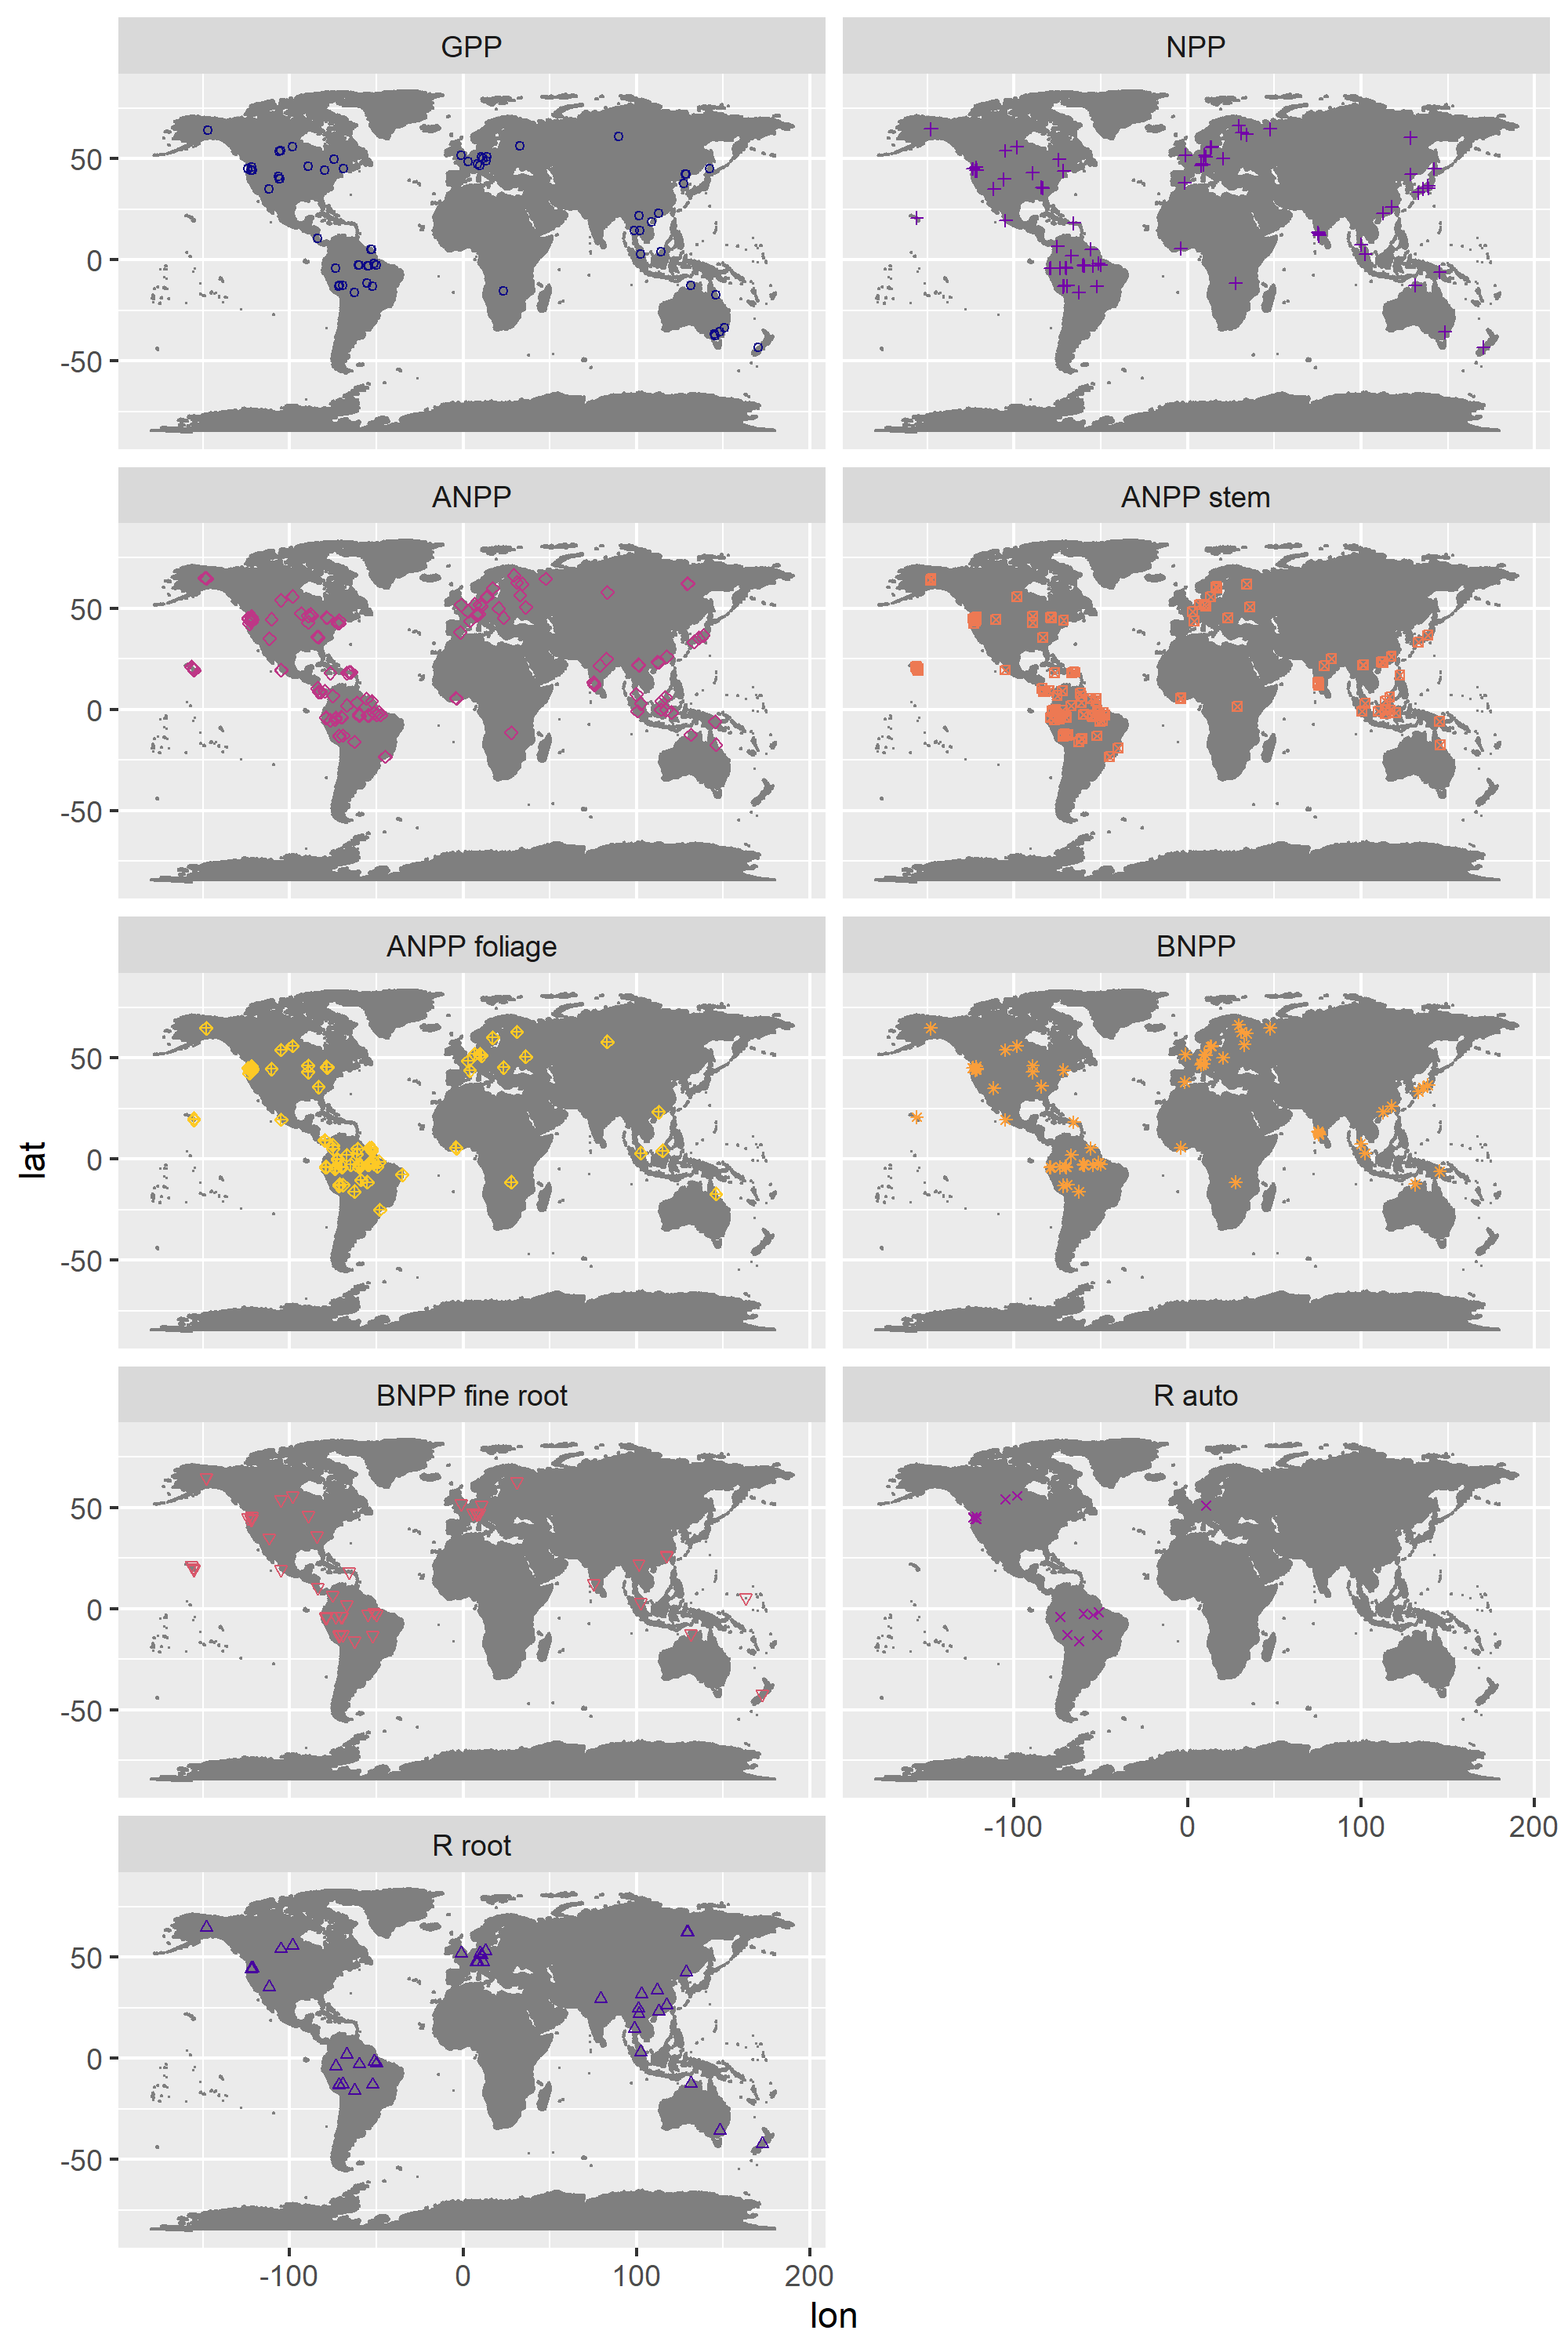
\includegraphics[width=27.78in,height=0.95\textheight]{tables_figures/distribution_all_samples} \caption{Figure S1: Maps showing distribution of samples for the nine FACF analyzed here.}\label{fig:unnamed-chunk-7}
\end{figure}

\blandscape

\begin{figure}[H]

{\centering 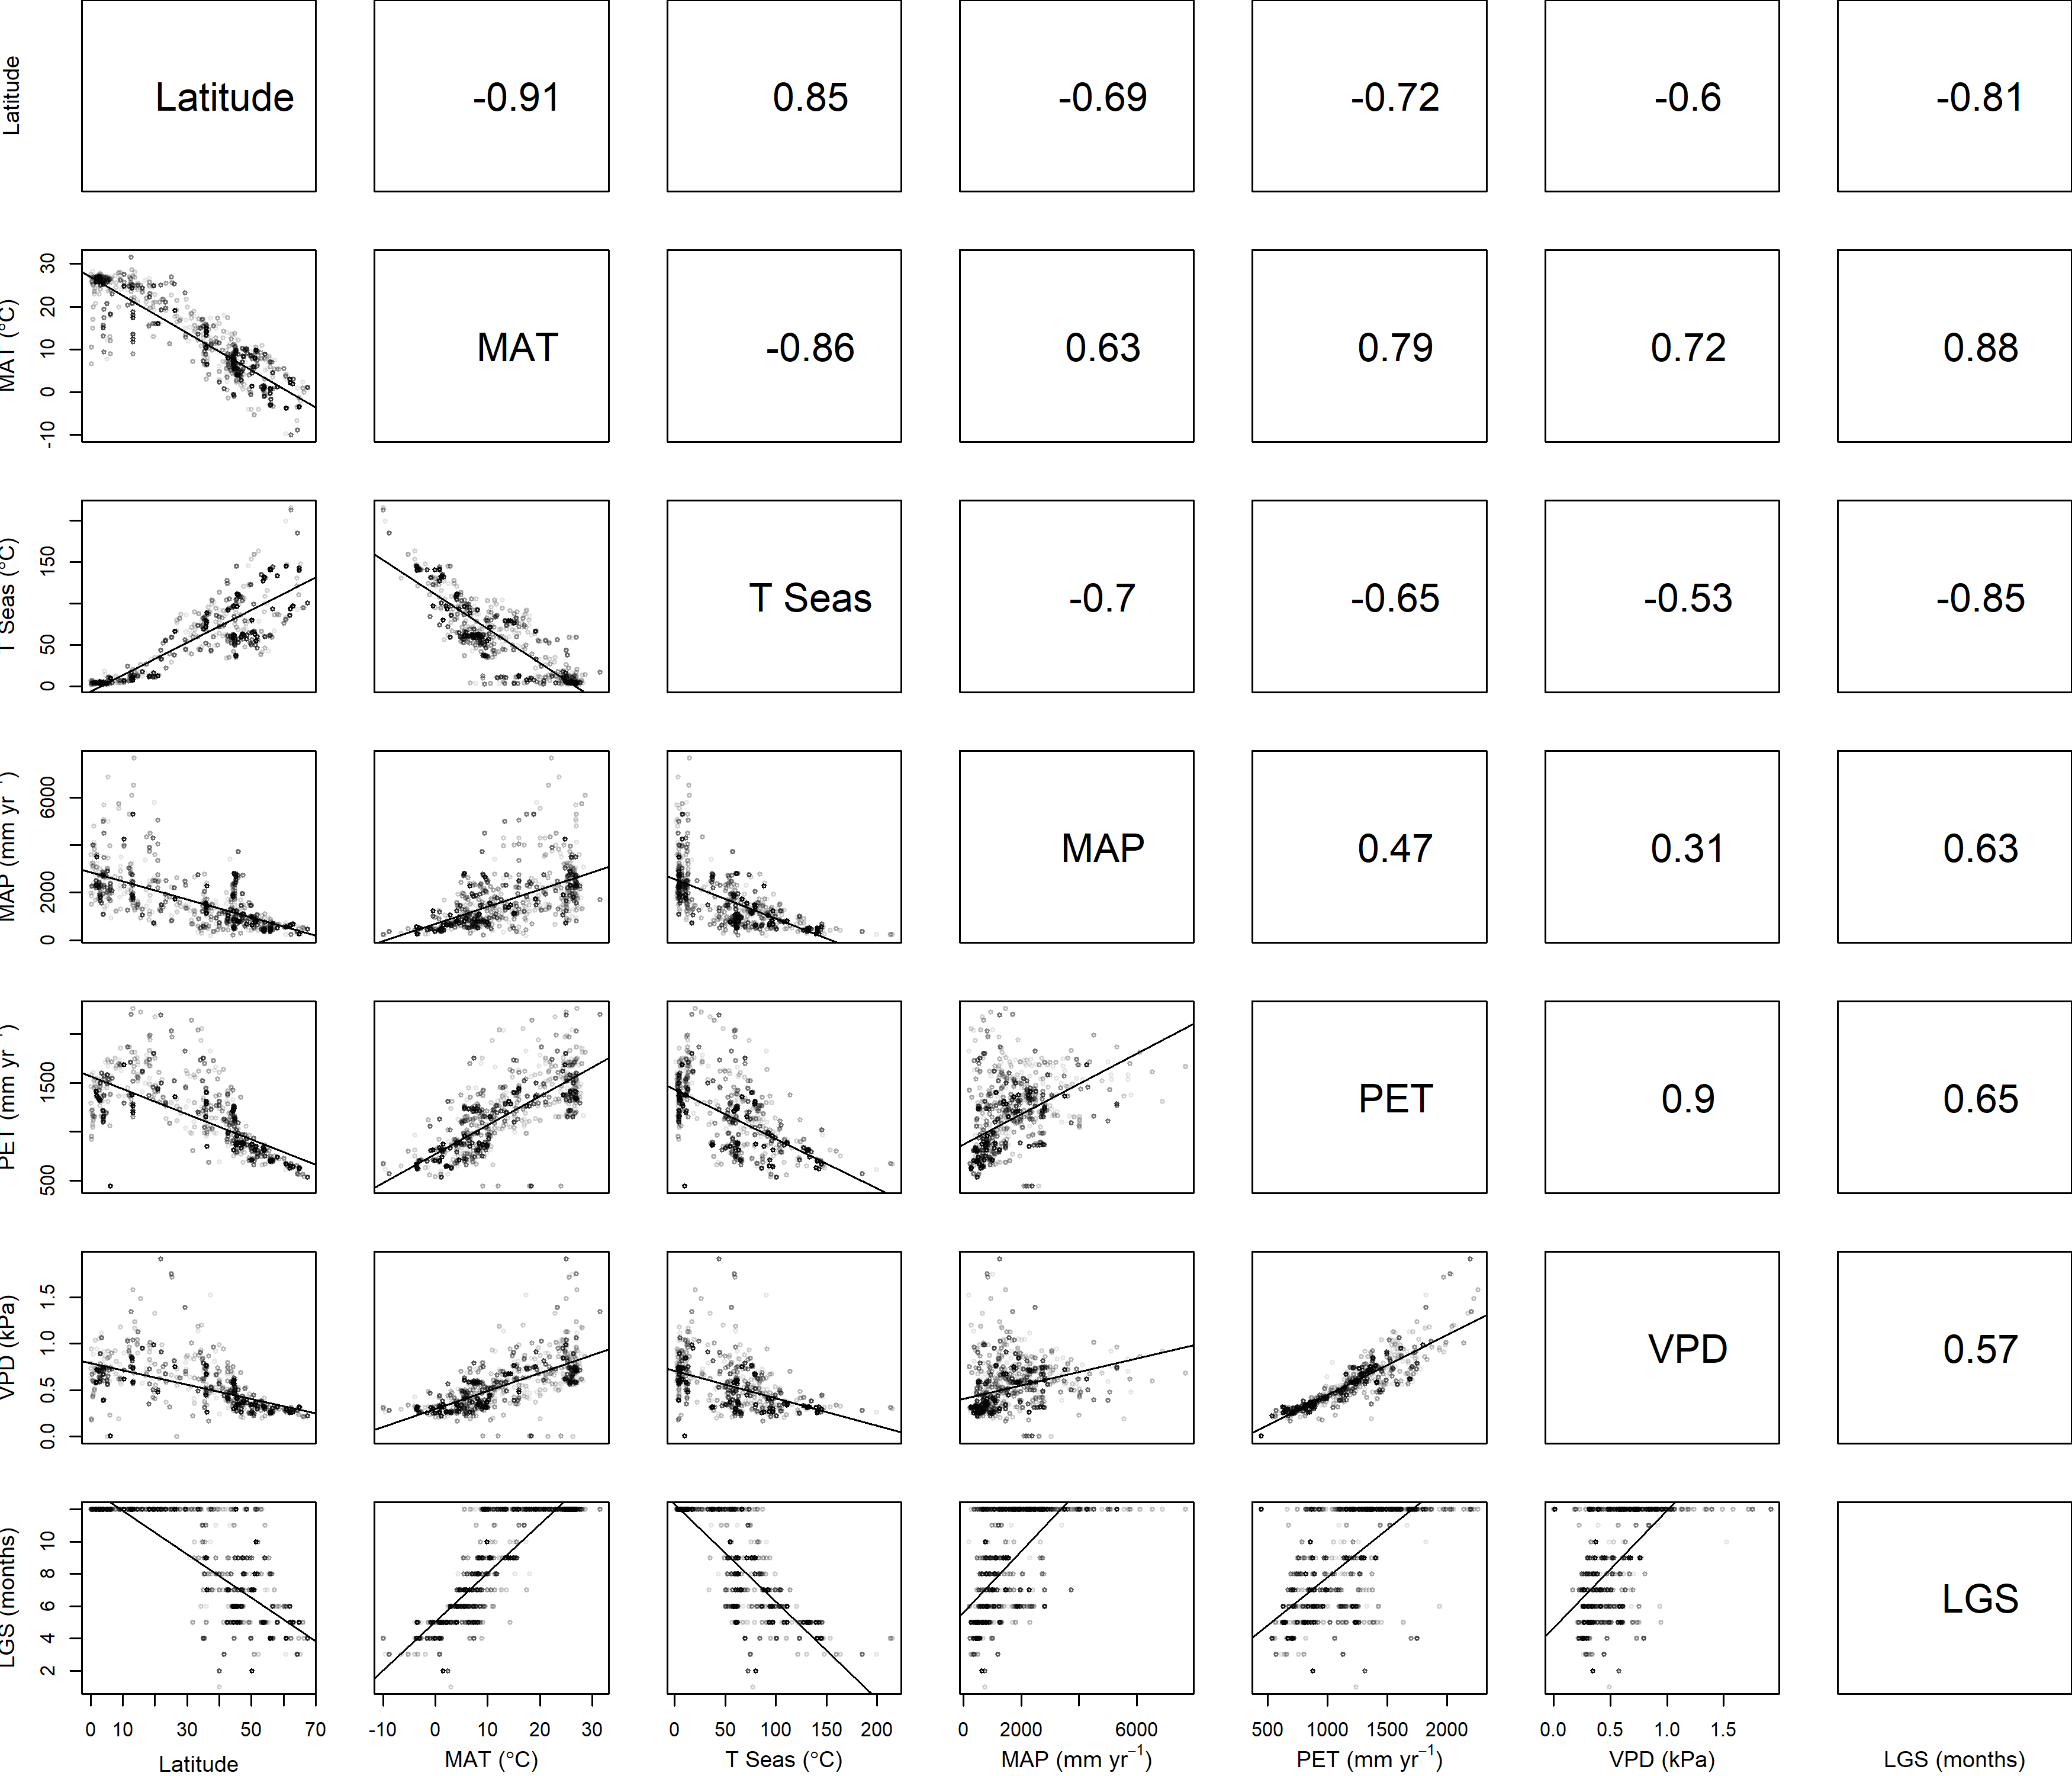
\includegraphics[width=48.61in,height=0.95\textheight]{tables_figures/climate_regressions} 

}

\caption{Figure S2: Correlations among latitude and climate variables. Variable names and units given in Table S1}\label{fig:unnamed-chunk-8}
\end{figure}

\elandscape

\blandscape

\begin{figure}[H]
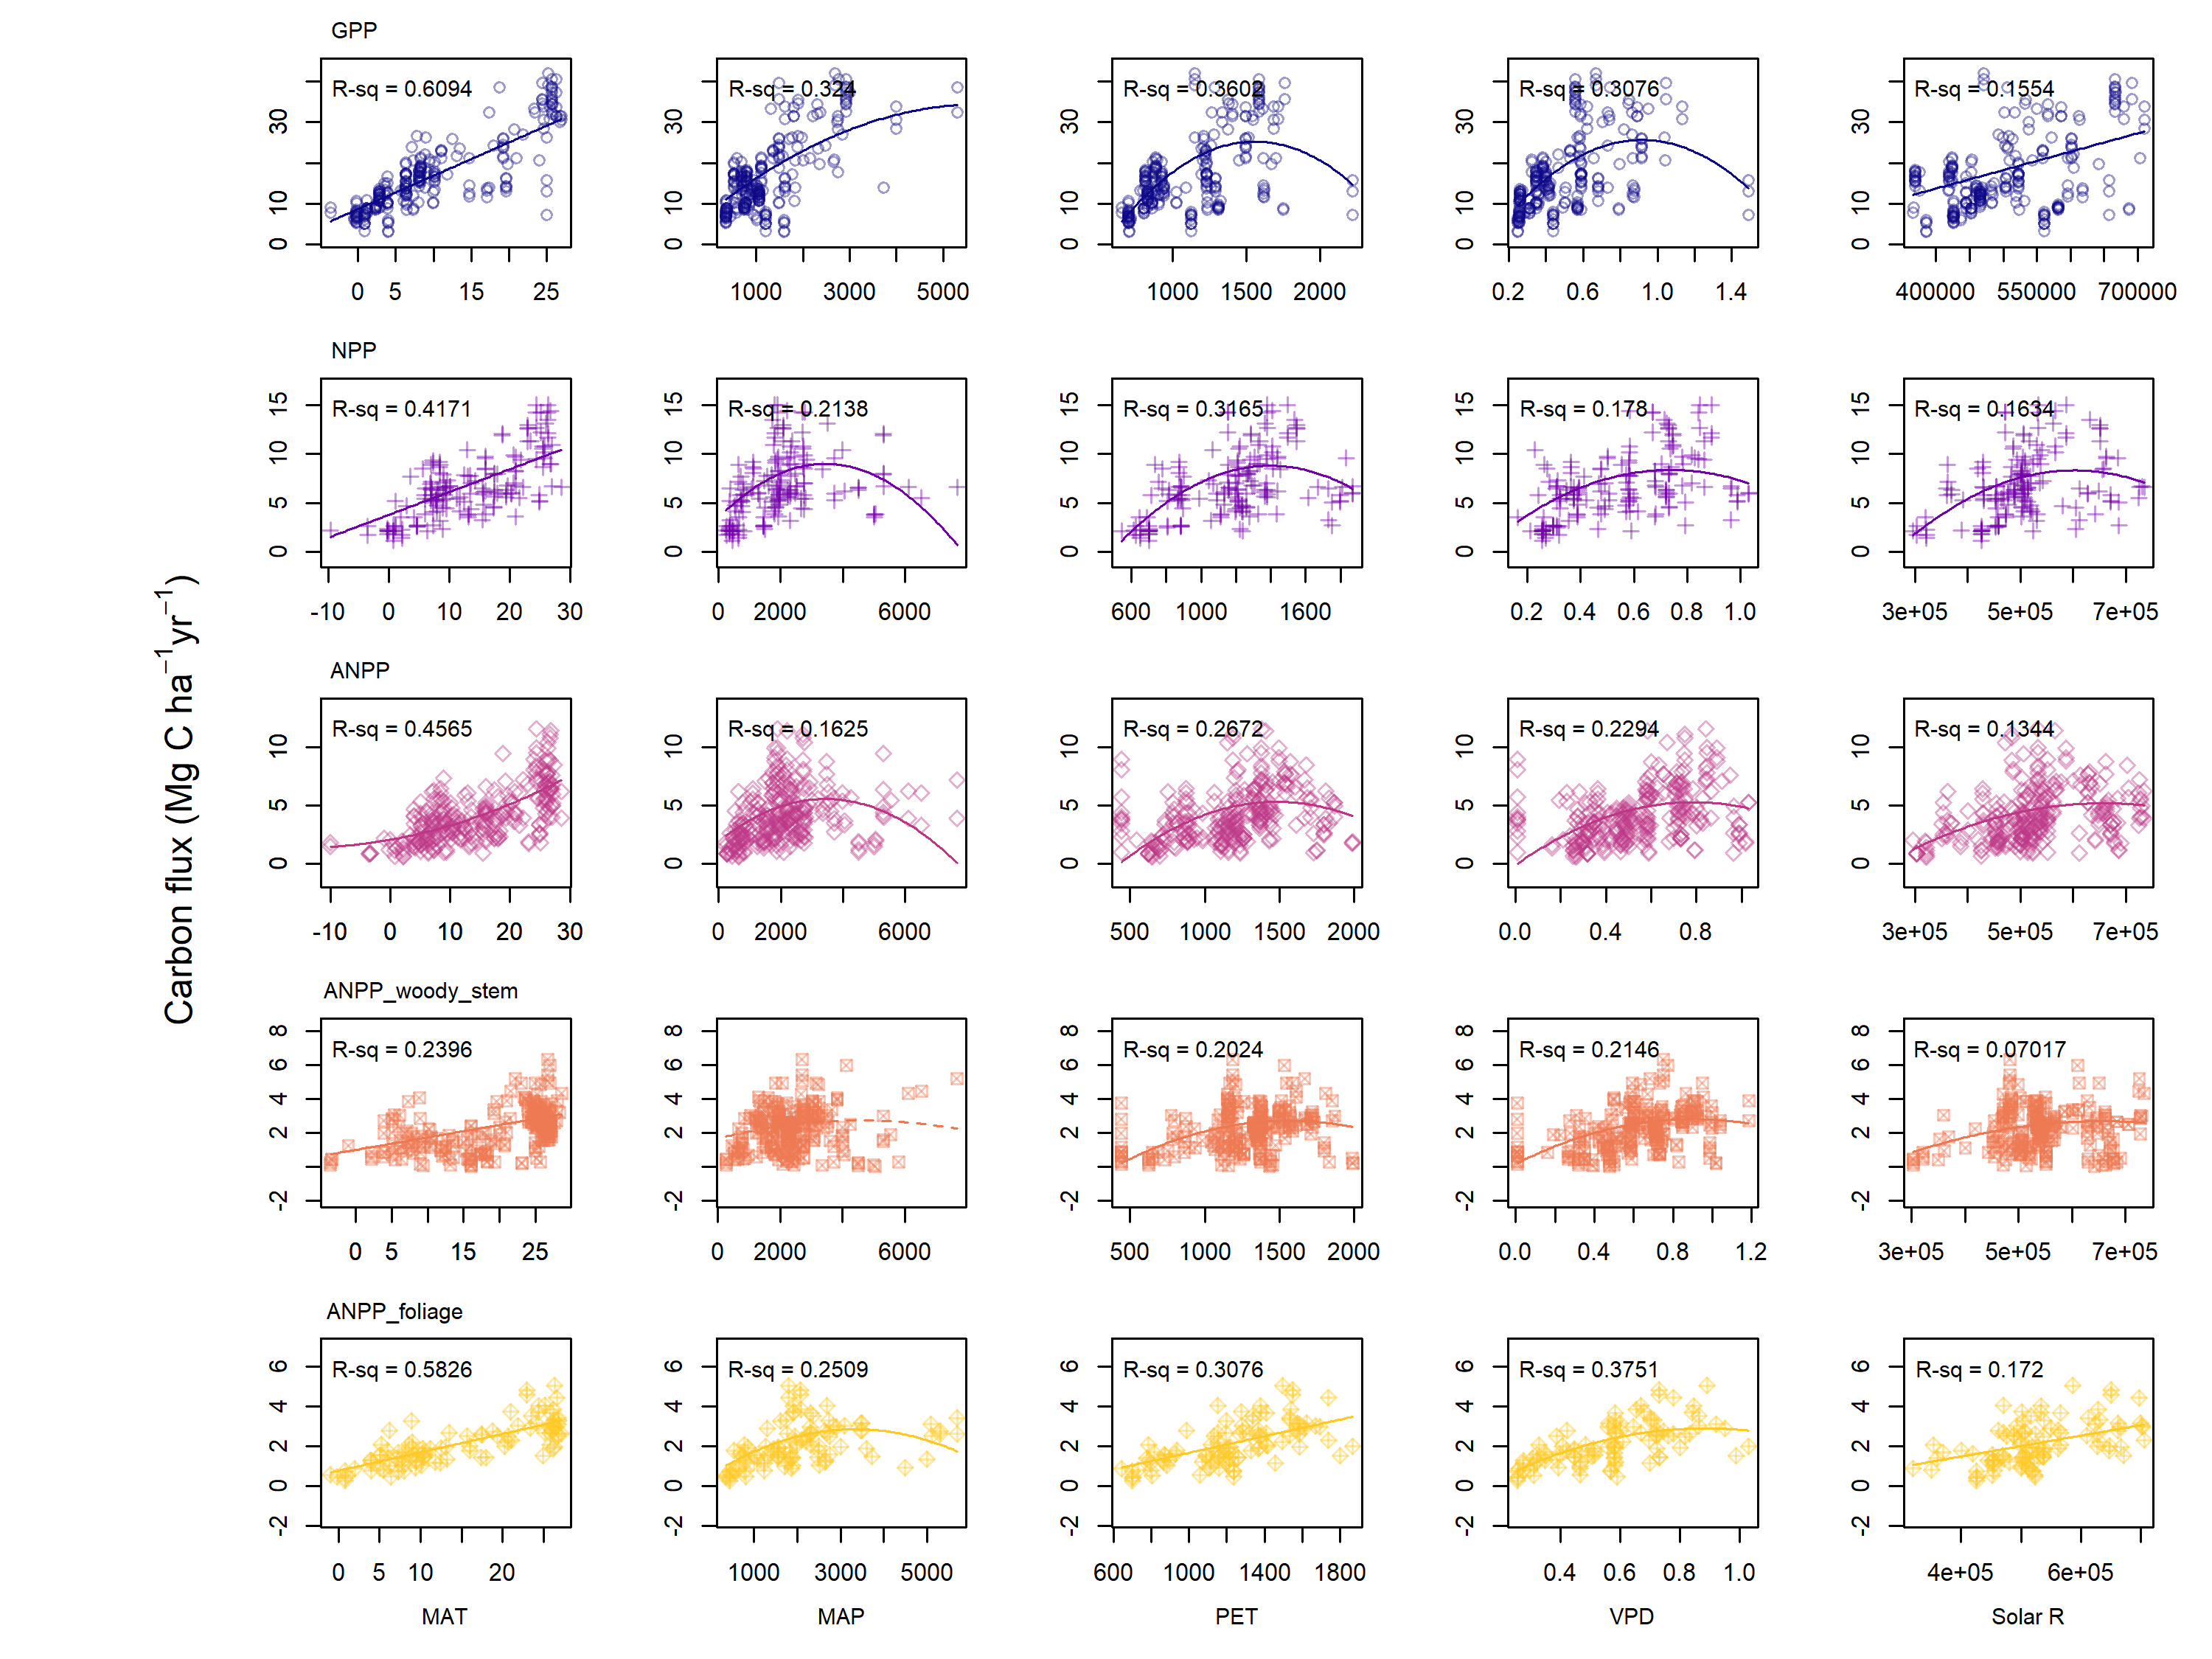
\includegraphics[width=41.67in,height=0.95\textheight]{tables_figures/grid_plots_climate1} \caption{Figure S3: Individual plots of FACF in relation to mean annual climate, part 1.}\label{fig:unnamed-chunk-9}
\end{figure}

\newpage

\begin{figure}[H]
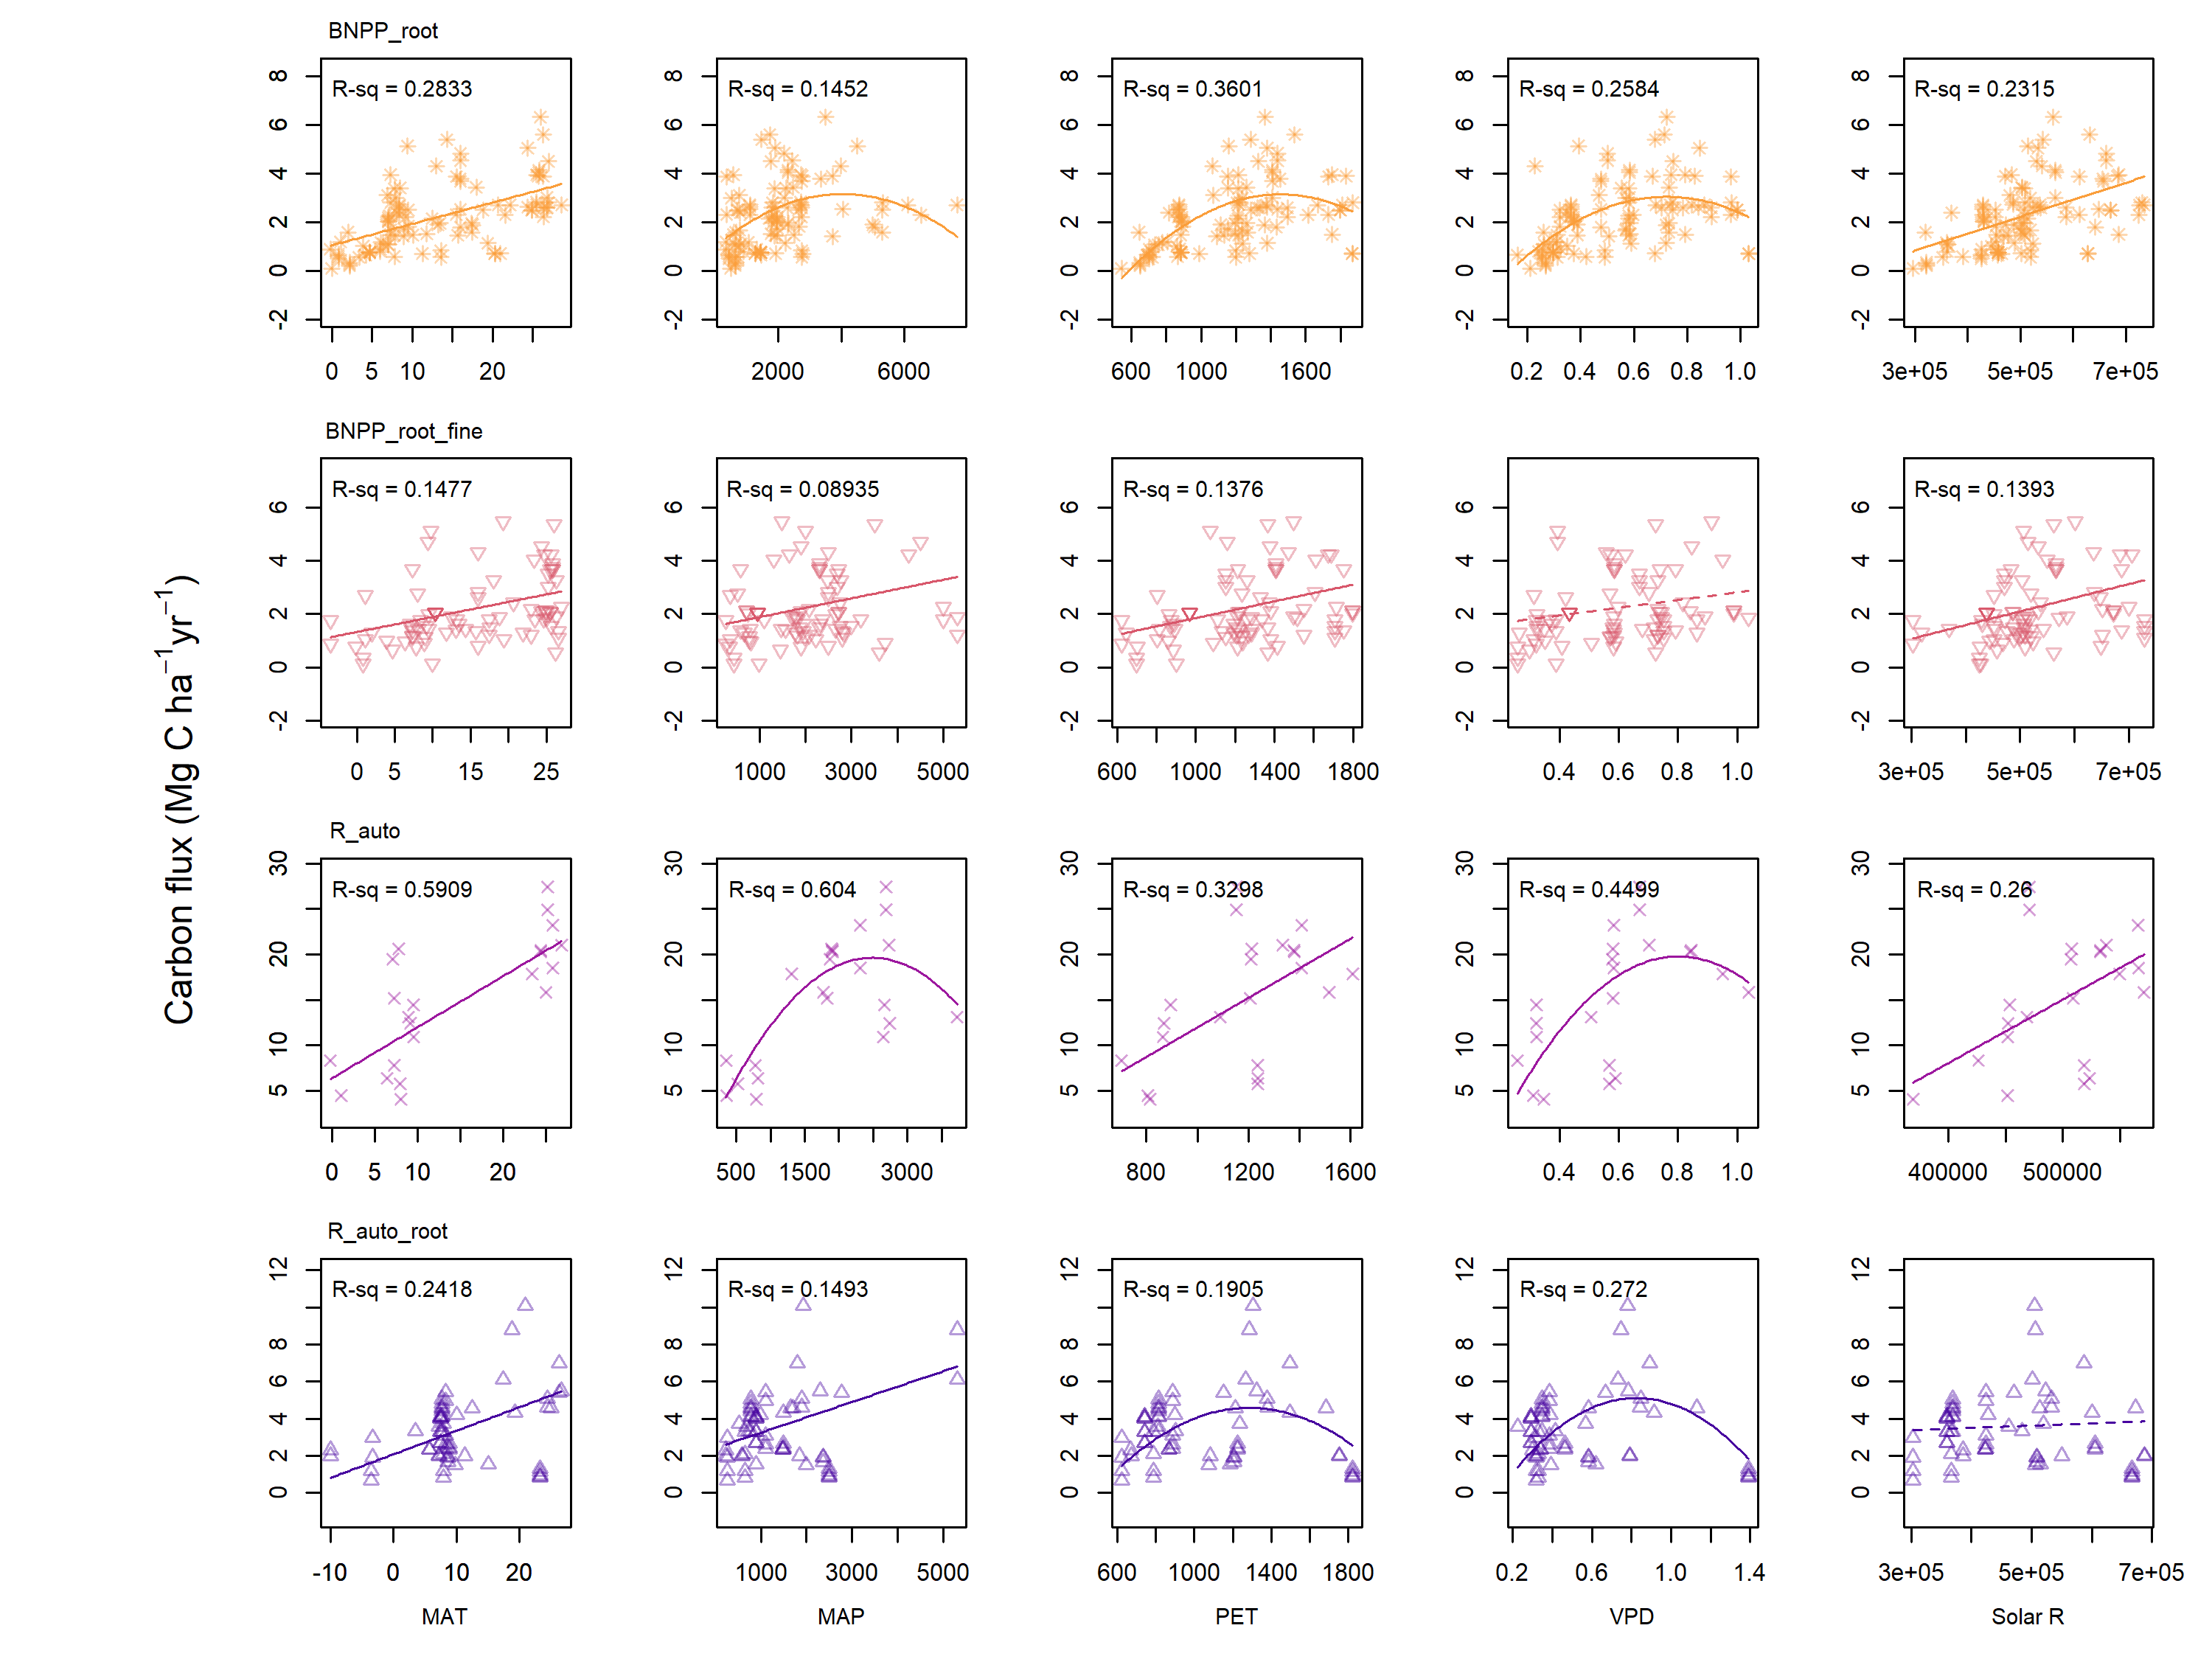
\includegraphics[width=41.67in,height=0.95\textheight]{tables_figures/grid_plots_climate2} \caption{Figure S4: Individual plots of FACF in relation to mean annual climate, part 2.}\label{fig:unnamed-chunk-10}
\end{figure}

\elandscape

\begin{figure}[H]
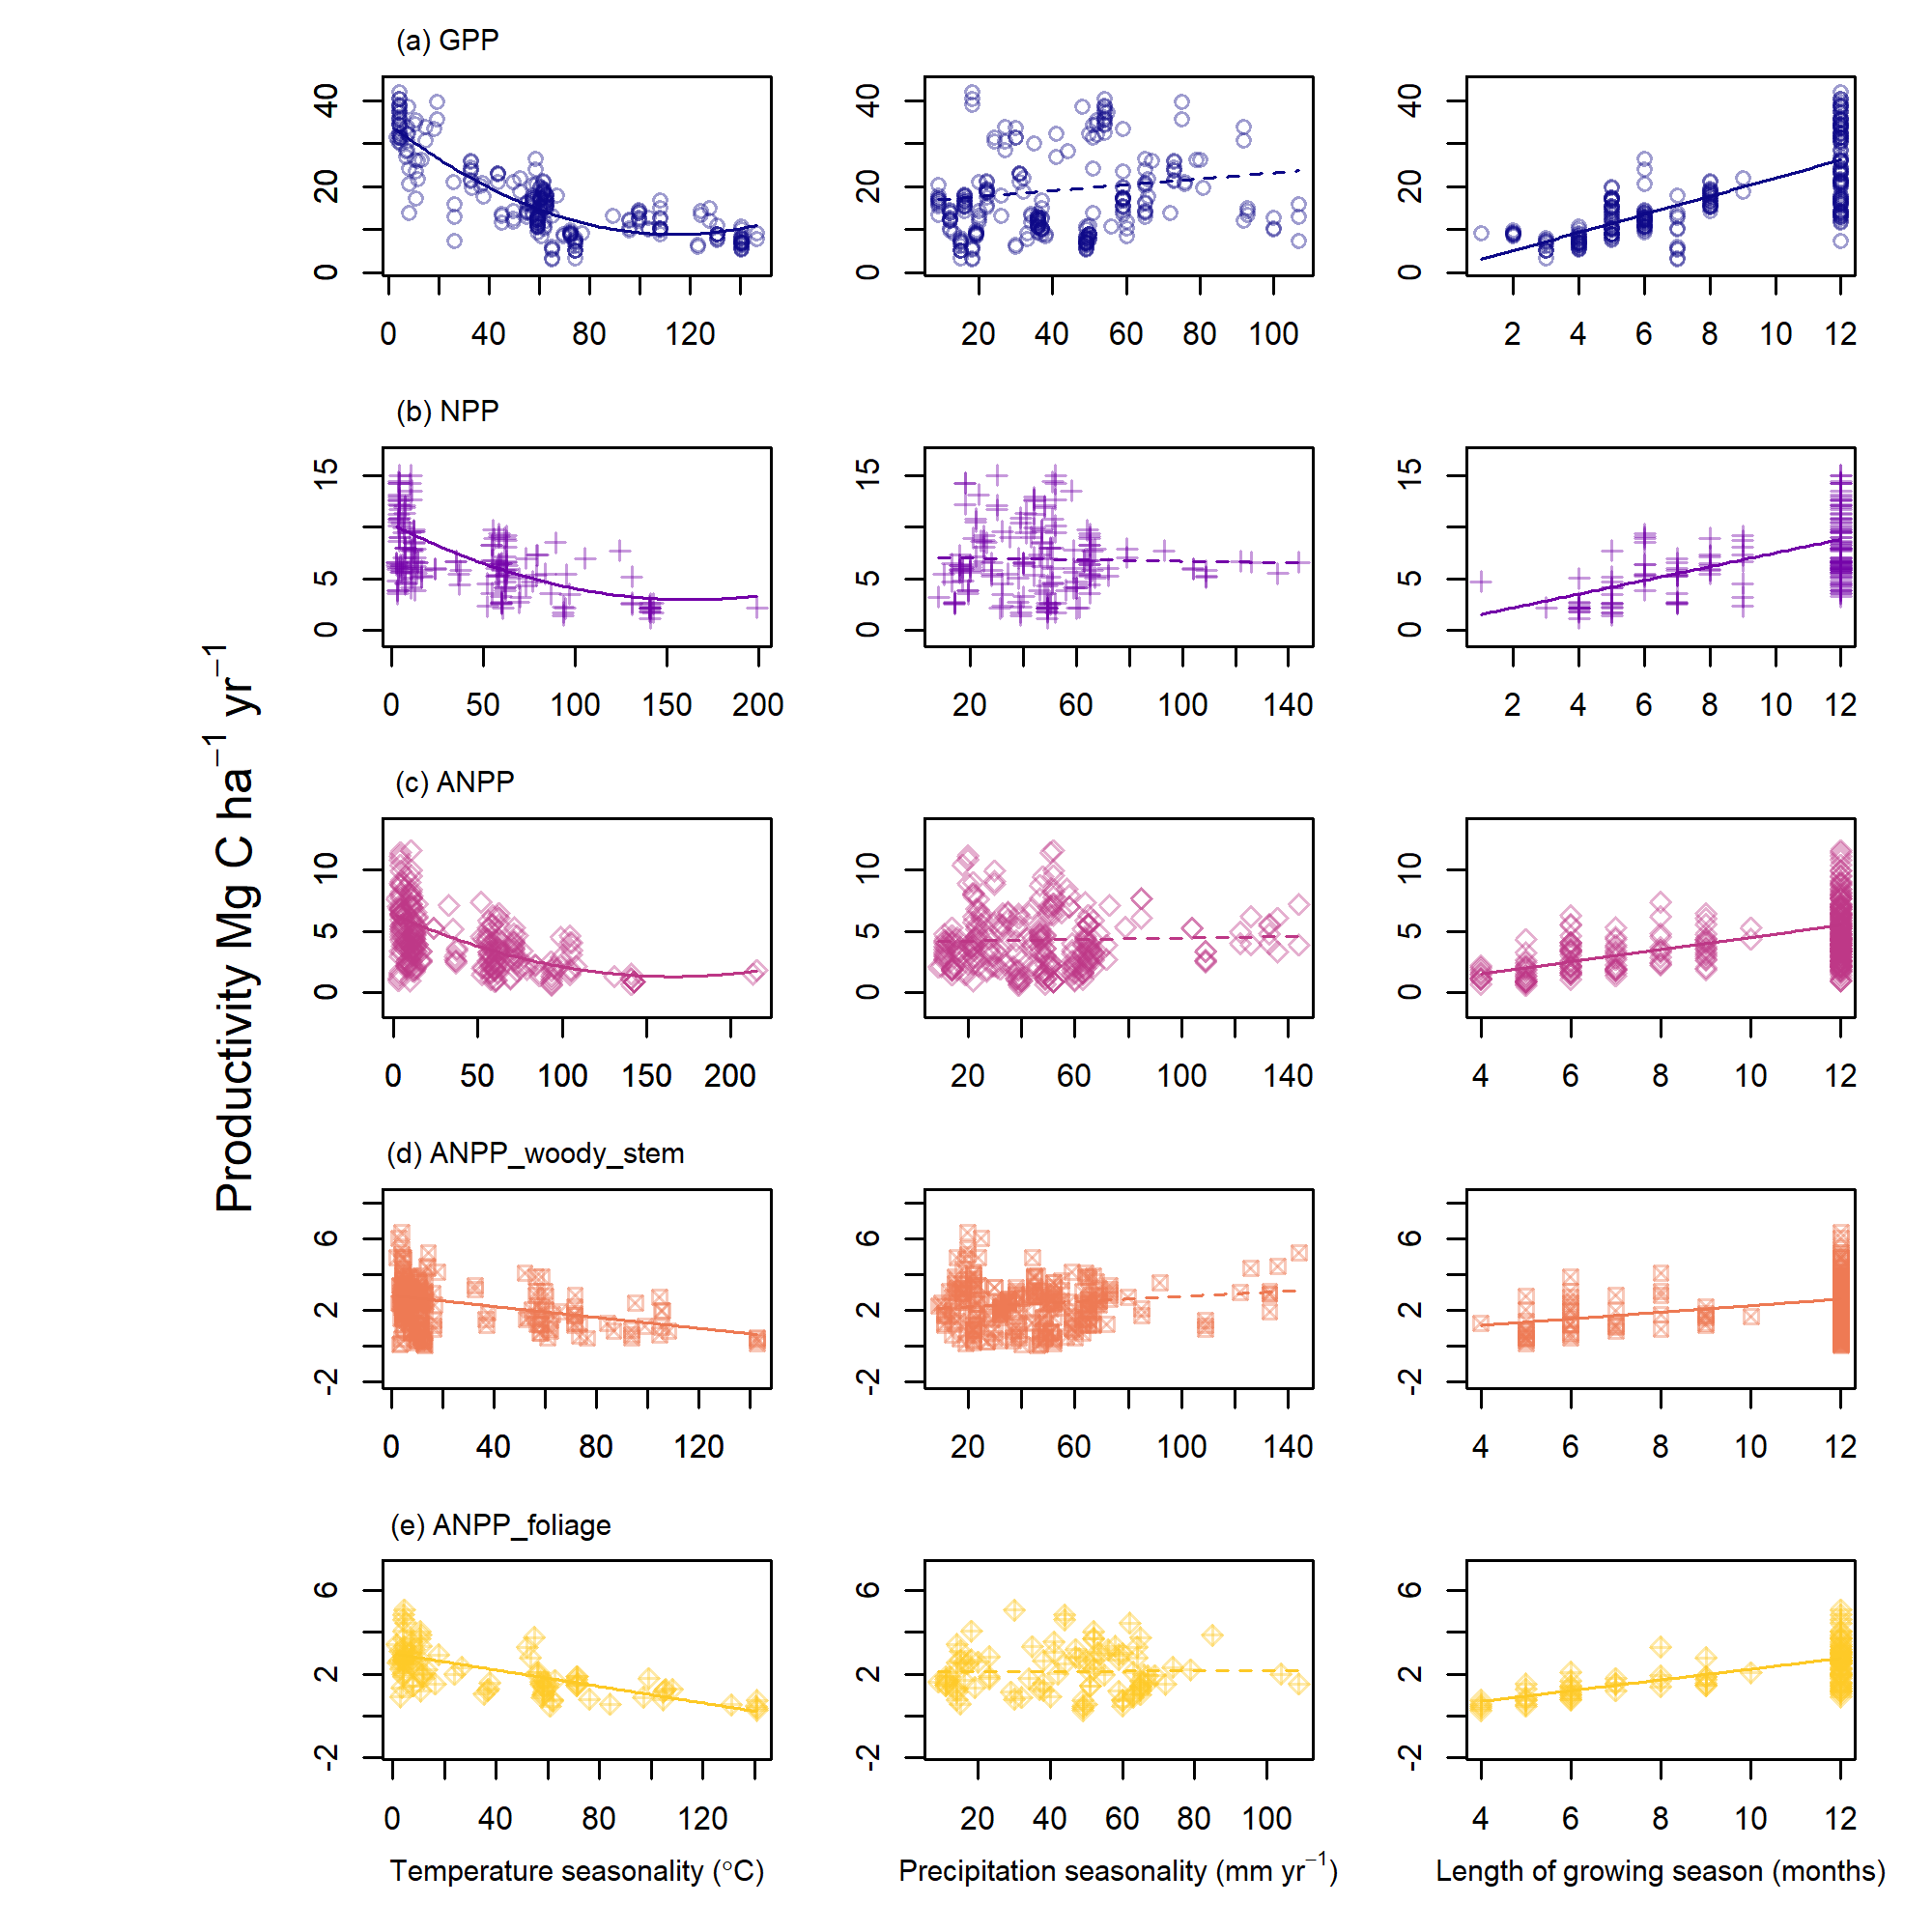
\includegraphics[width=27.78in,height=0.95\textheight]{tables_figures/grid_plots_seasonality3} \caption{Figure S5: Individual plots of FACF in relation to mean climate seasonality, part 1.}\label{fig:unnamed-chunk-11}
\end{figure}

\newpage

\begin{figure}[H]
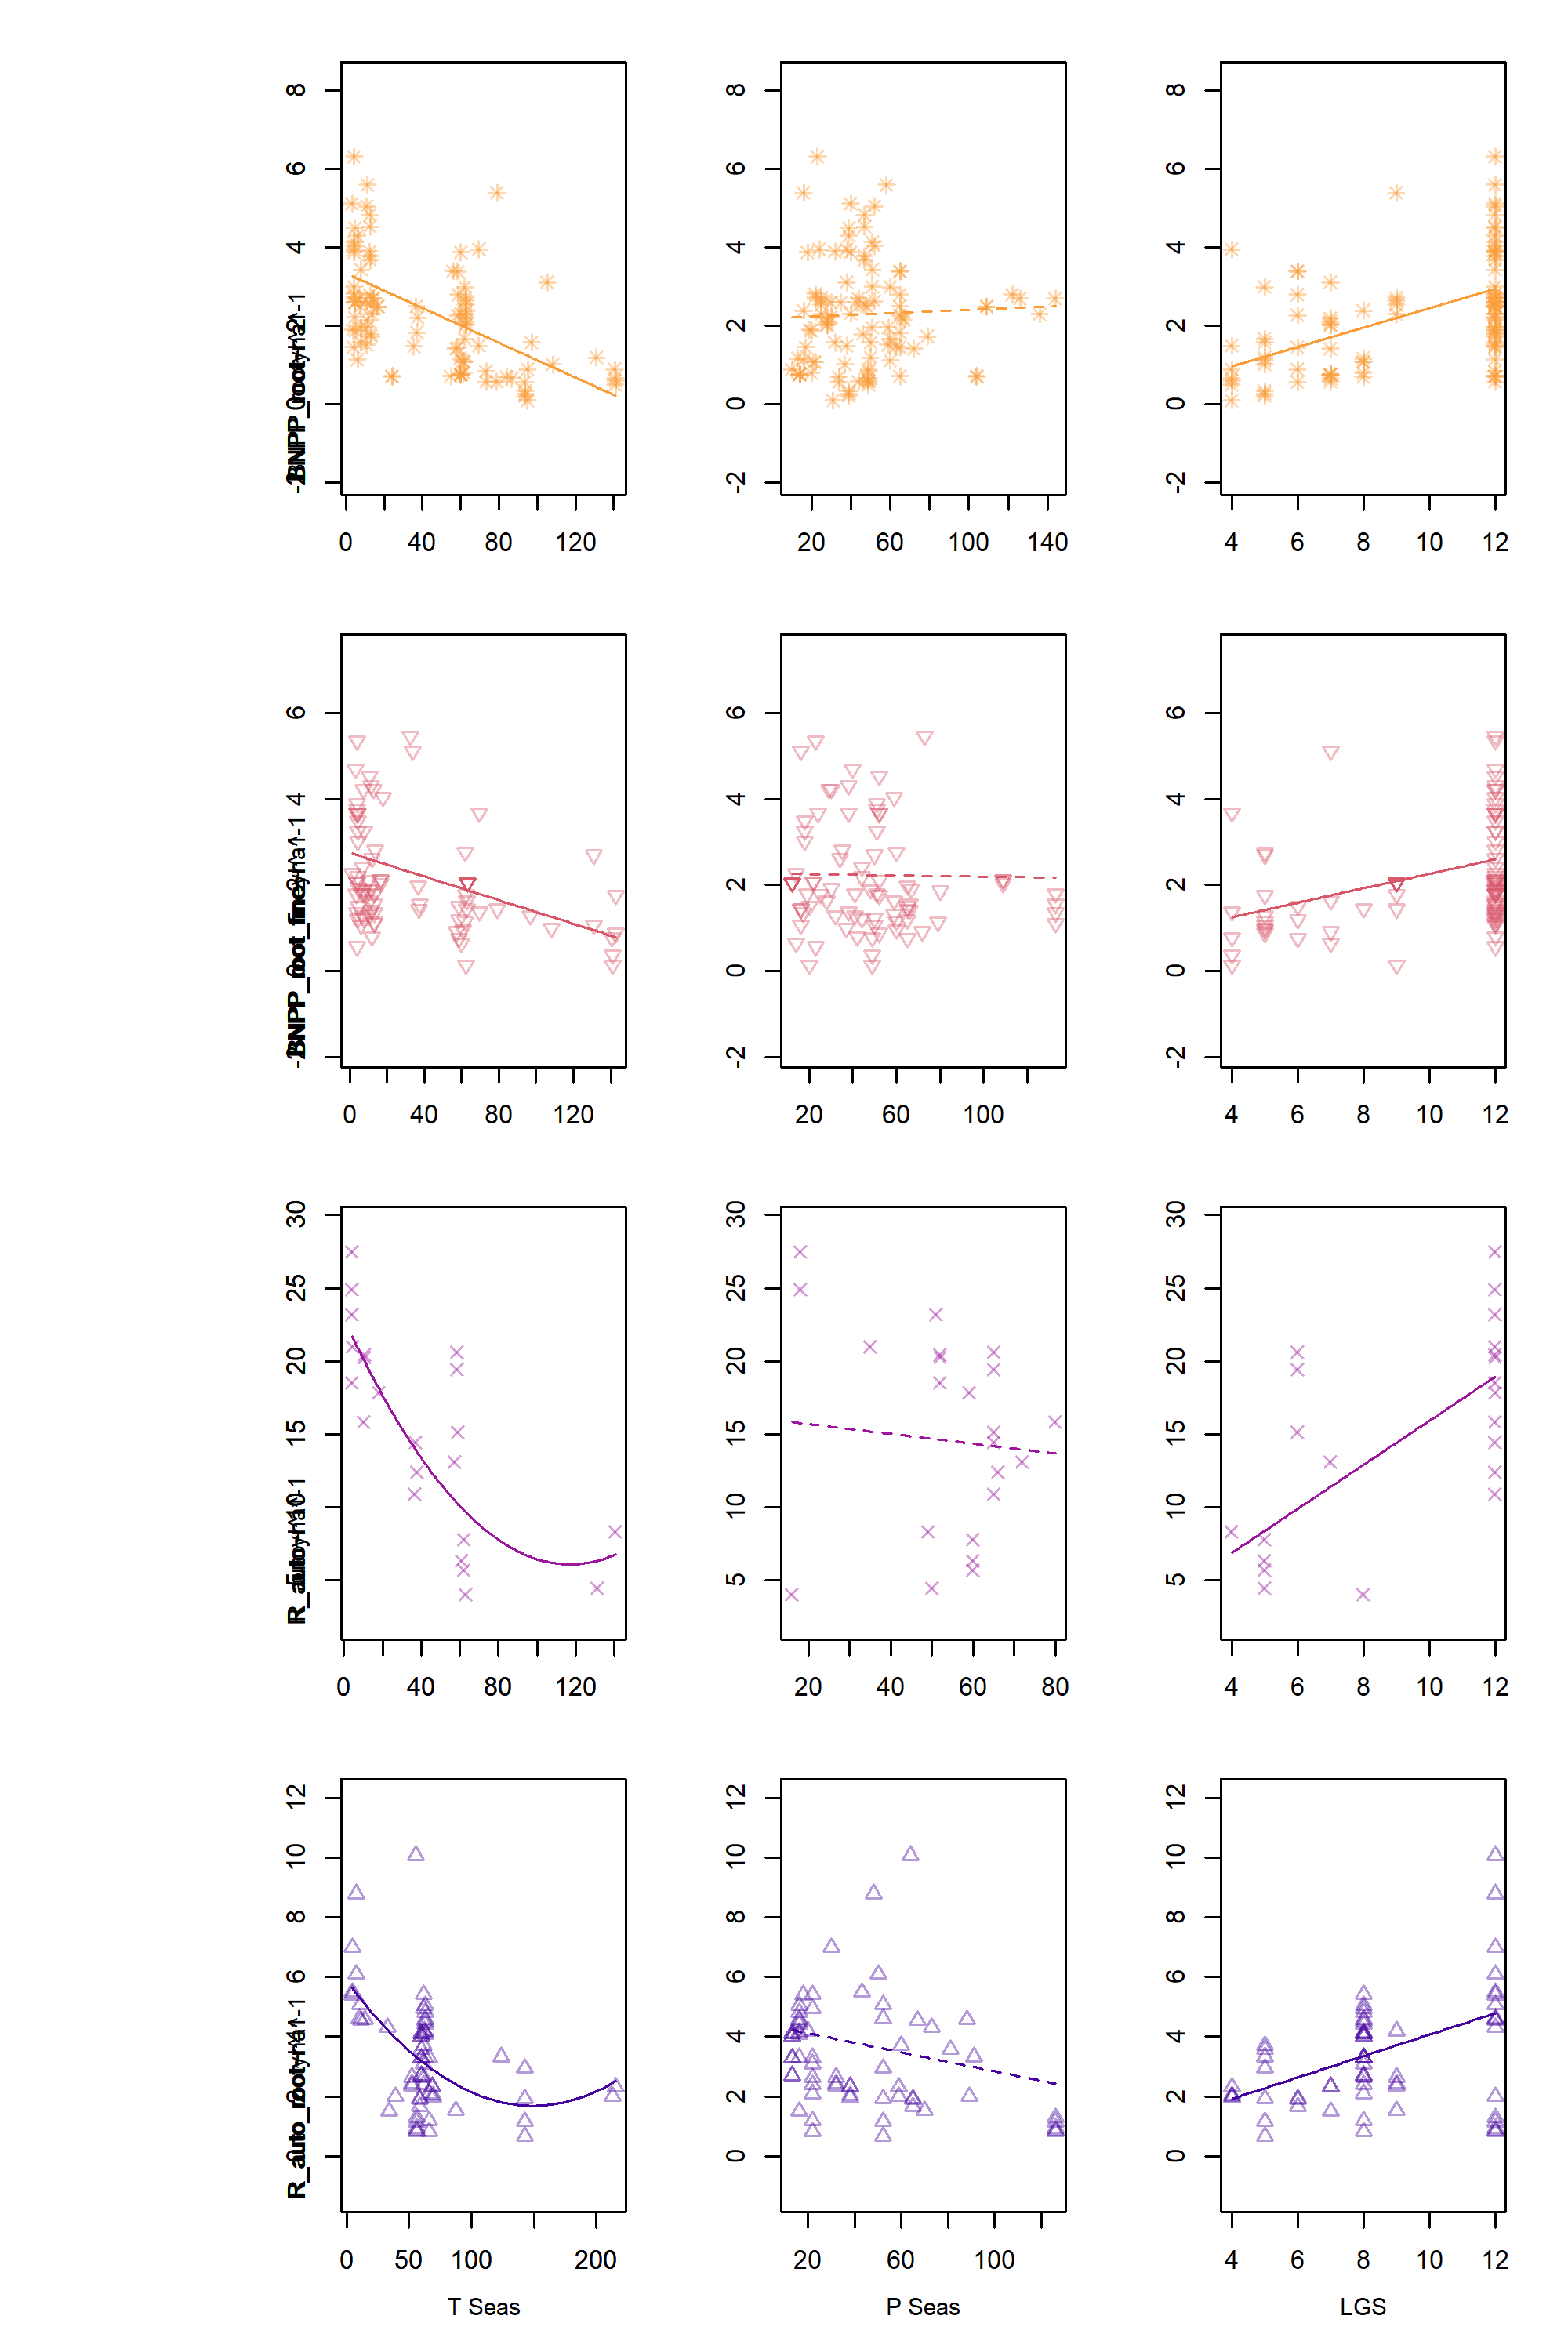
\includegraphics[width=1\linewidth]{tables_figures/grid_plots_seasonality4} \caption{Figure S6: Individual plots of FACF in relation to mean climate seasonality, part 2.}\label{fig:unnamed-chunk-12}
\end{figure}

\newpage

\begin{figure}[H]
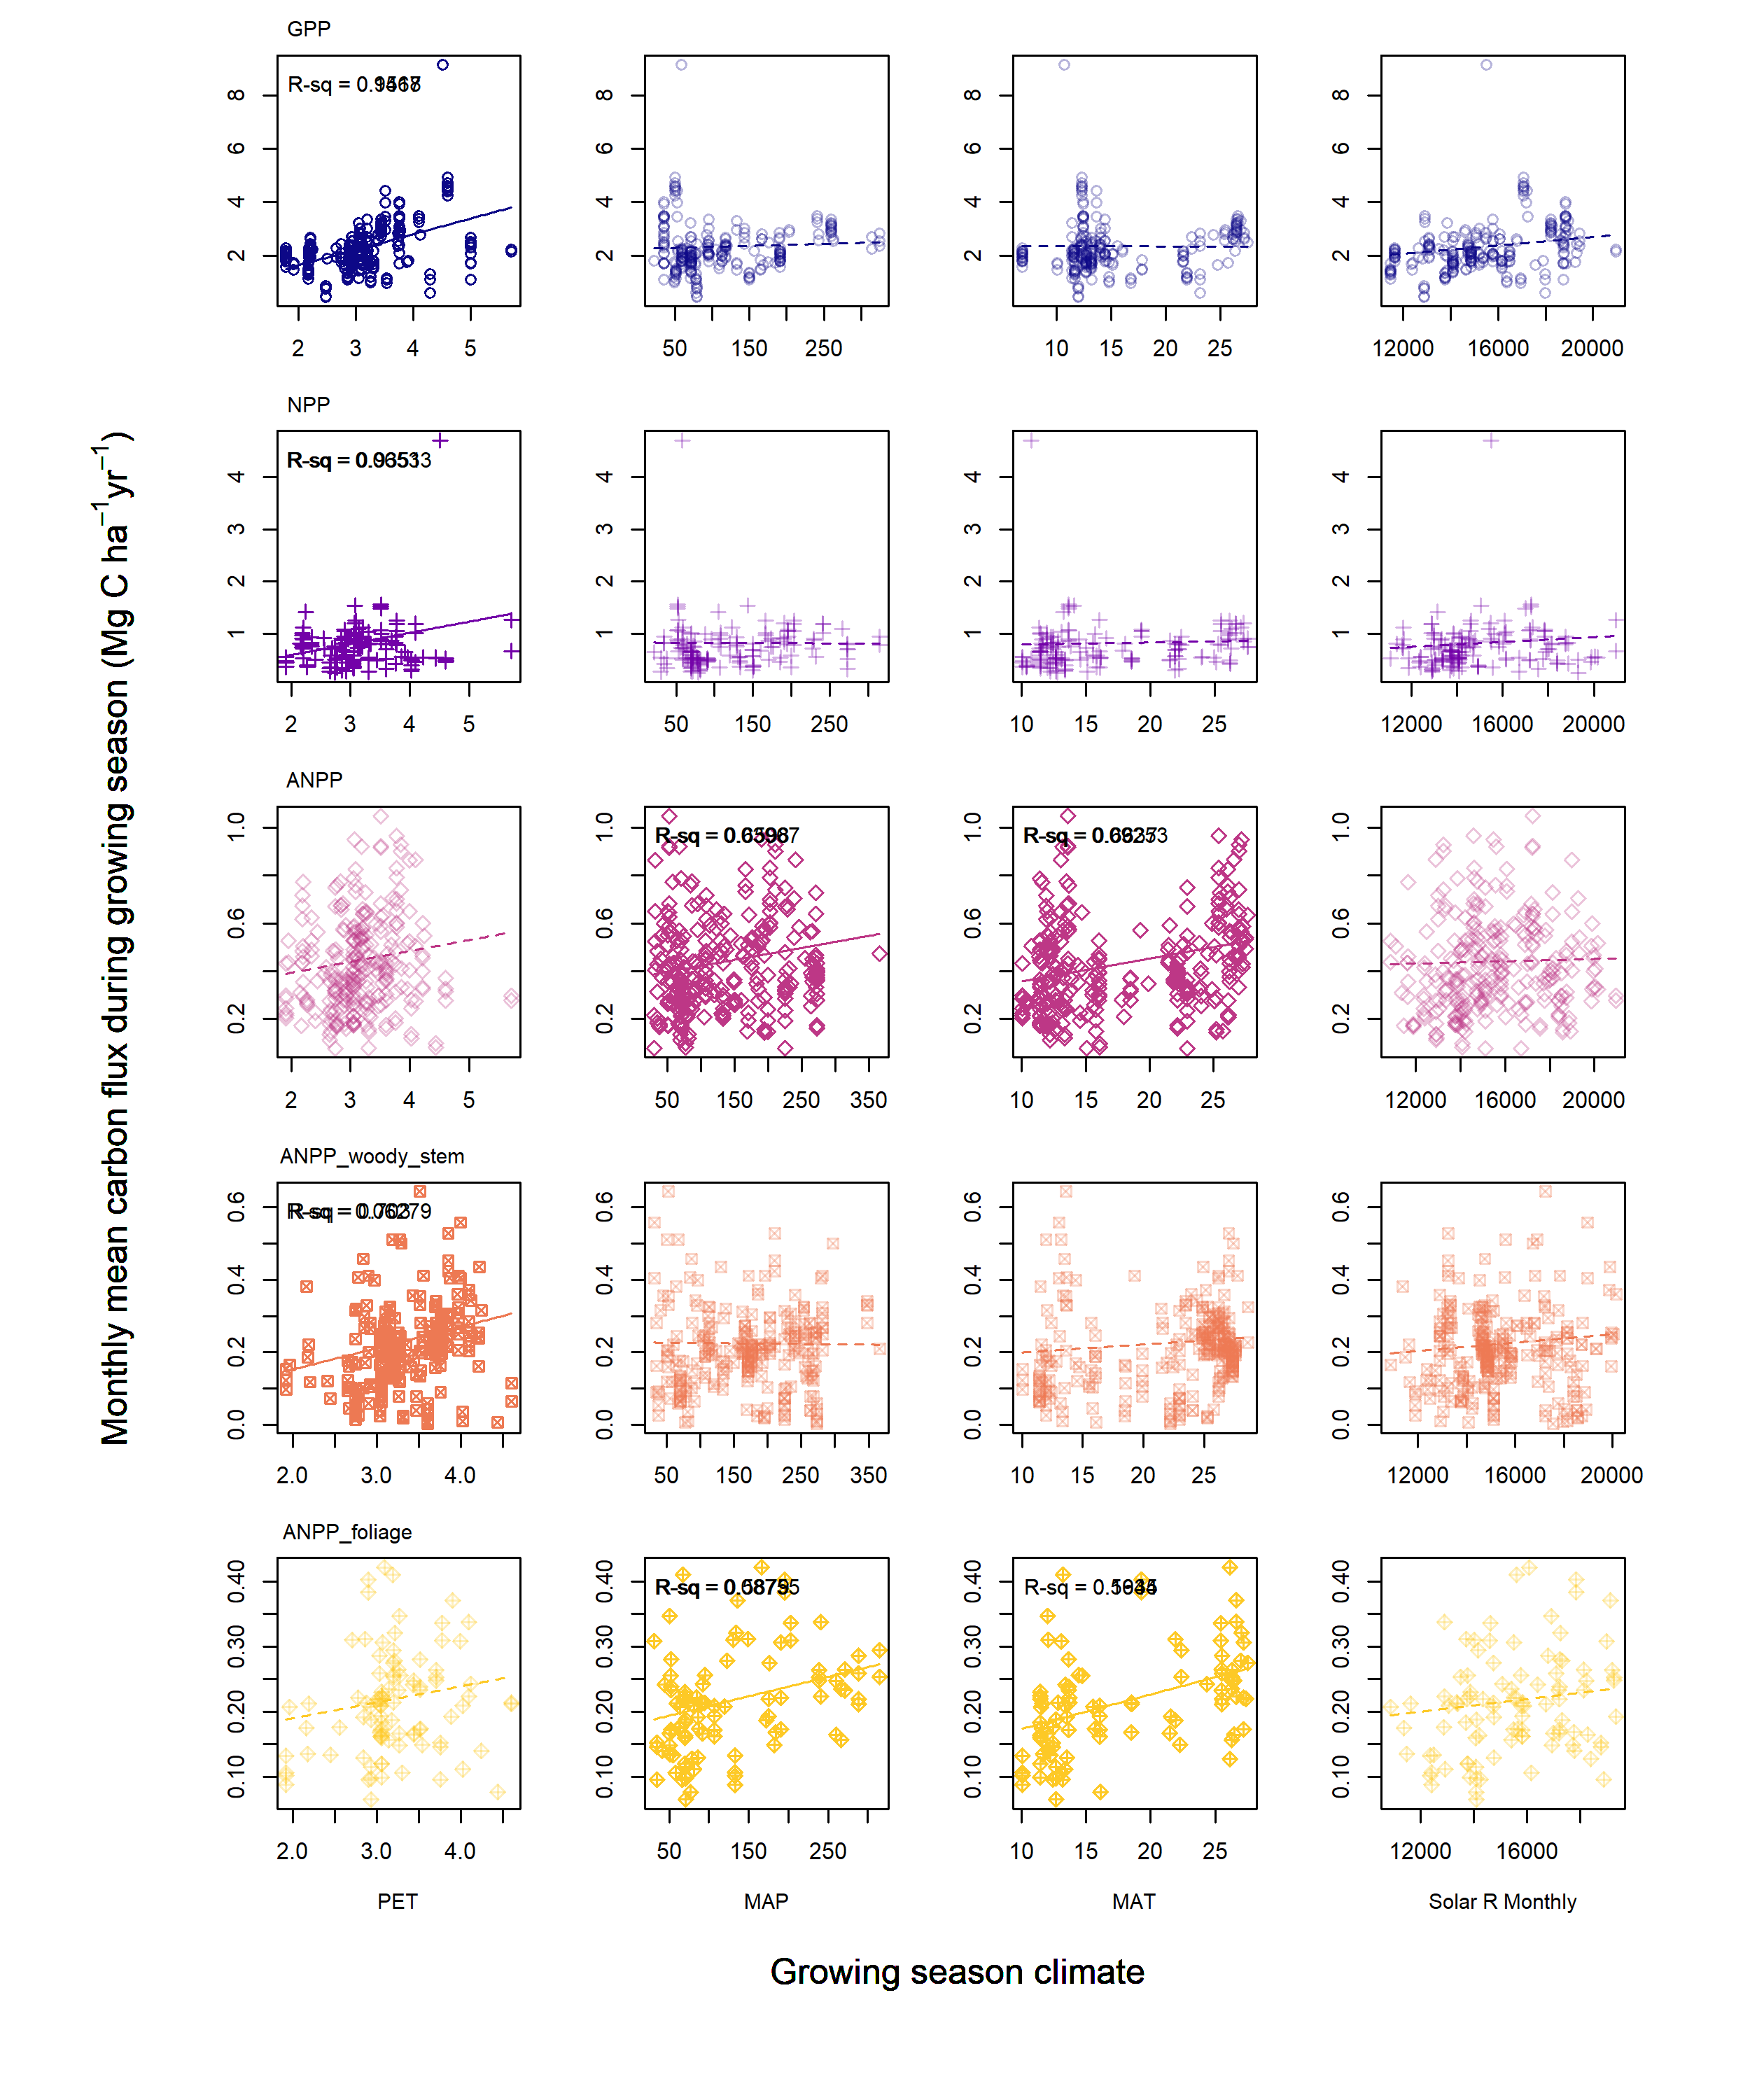
\includegraphics[width=1\linewidth]{tables_figures/gridded_growing_season1} \caption{Figure S7: Growing season length-standardized FACF in relation to mean growing season climate, part 1.}\label{fig:unnamed-chunk-13}
\end{figure}

\newpage

\begin{figure}[H]
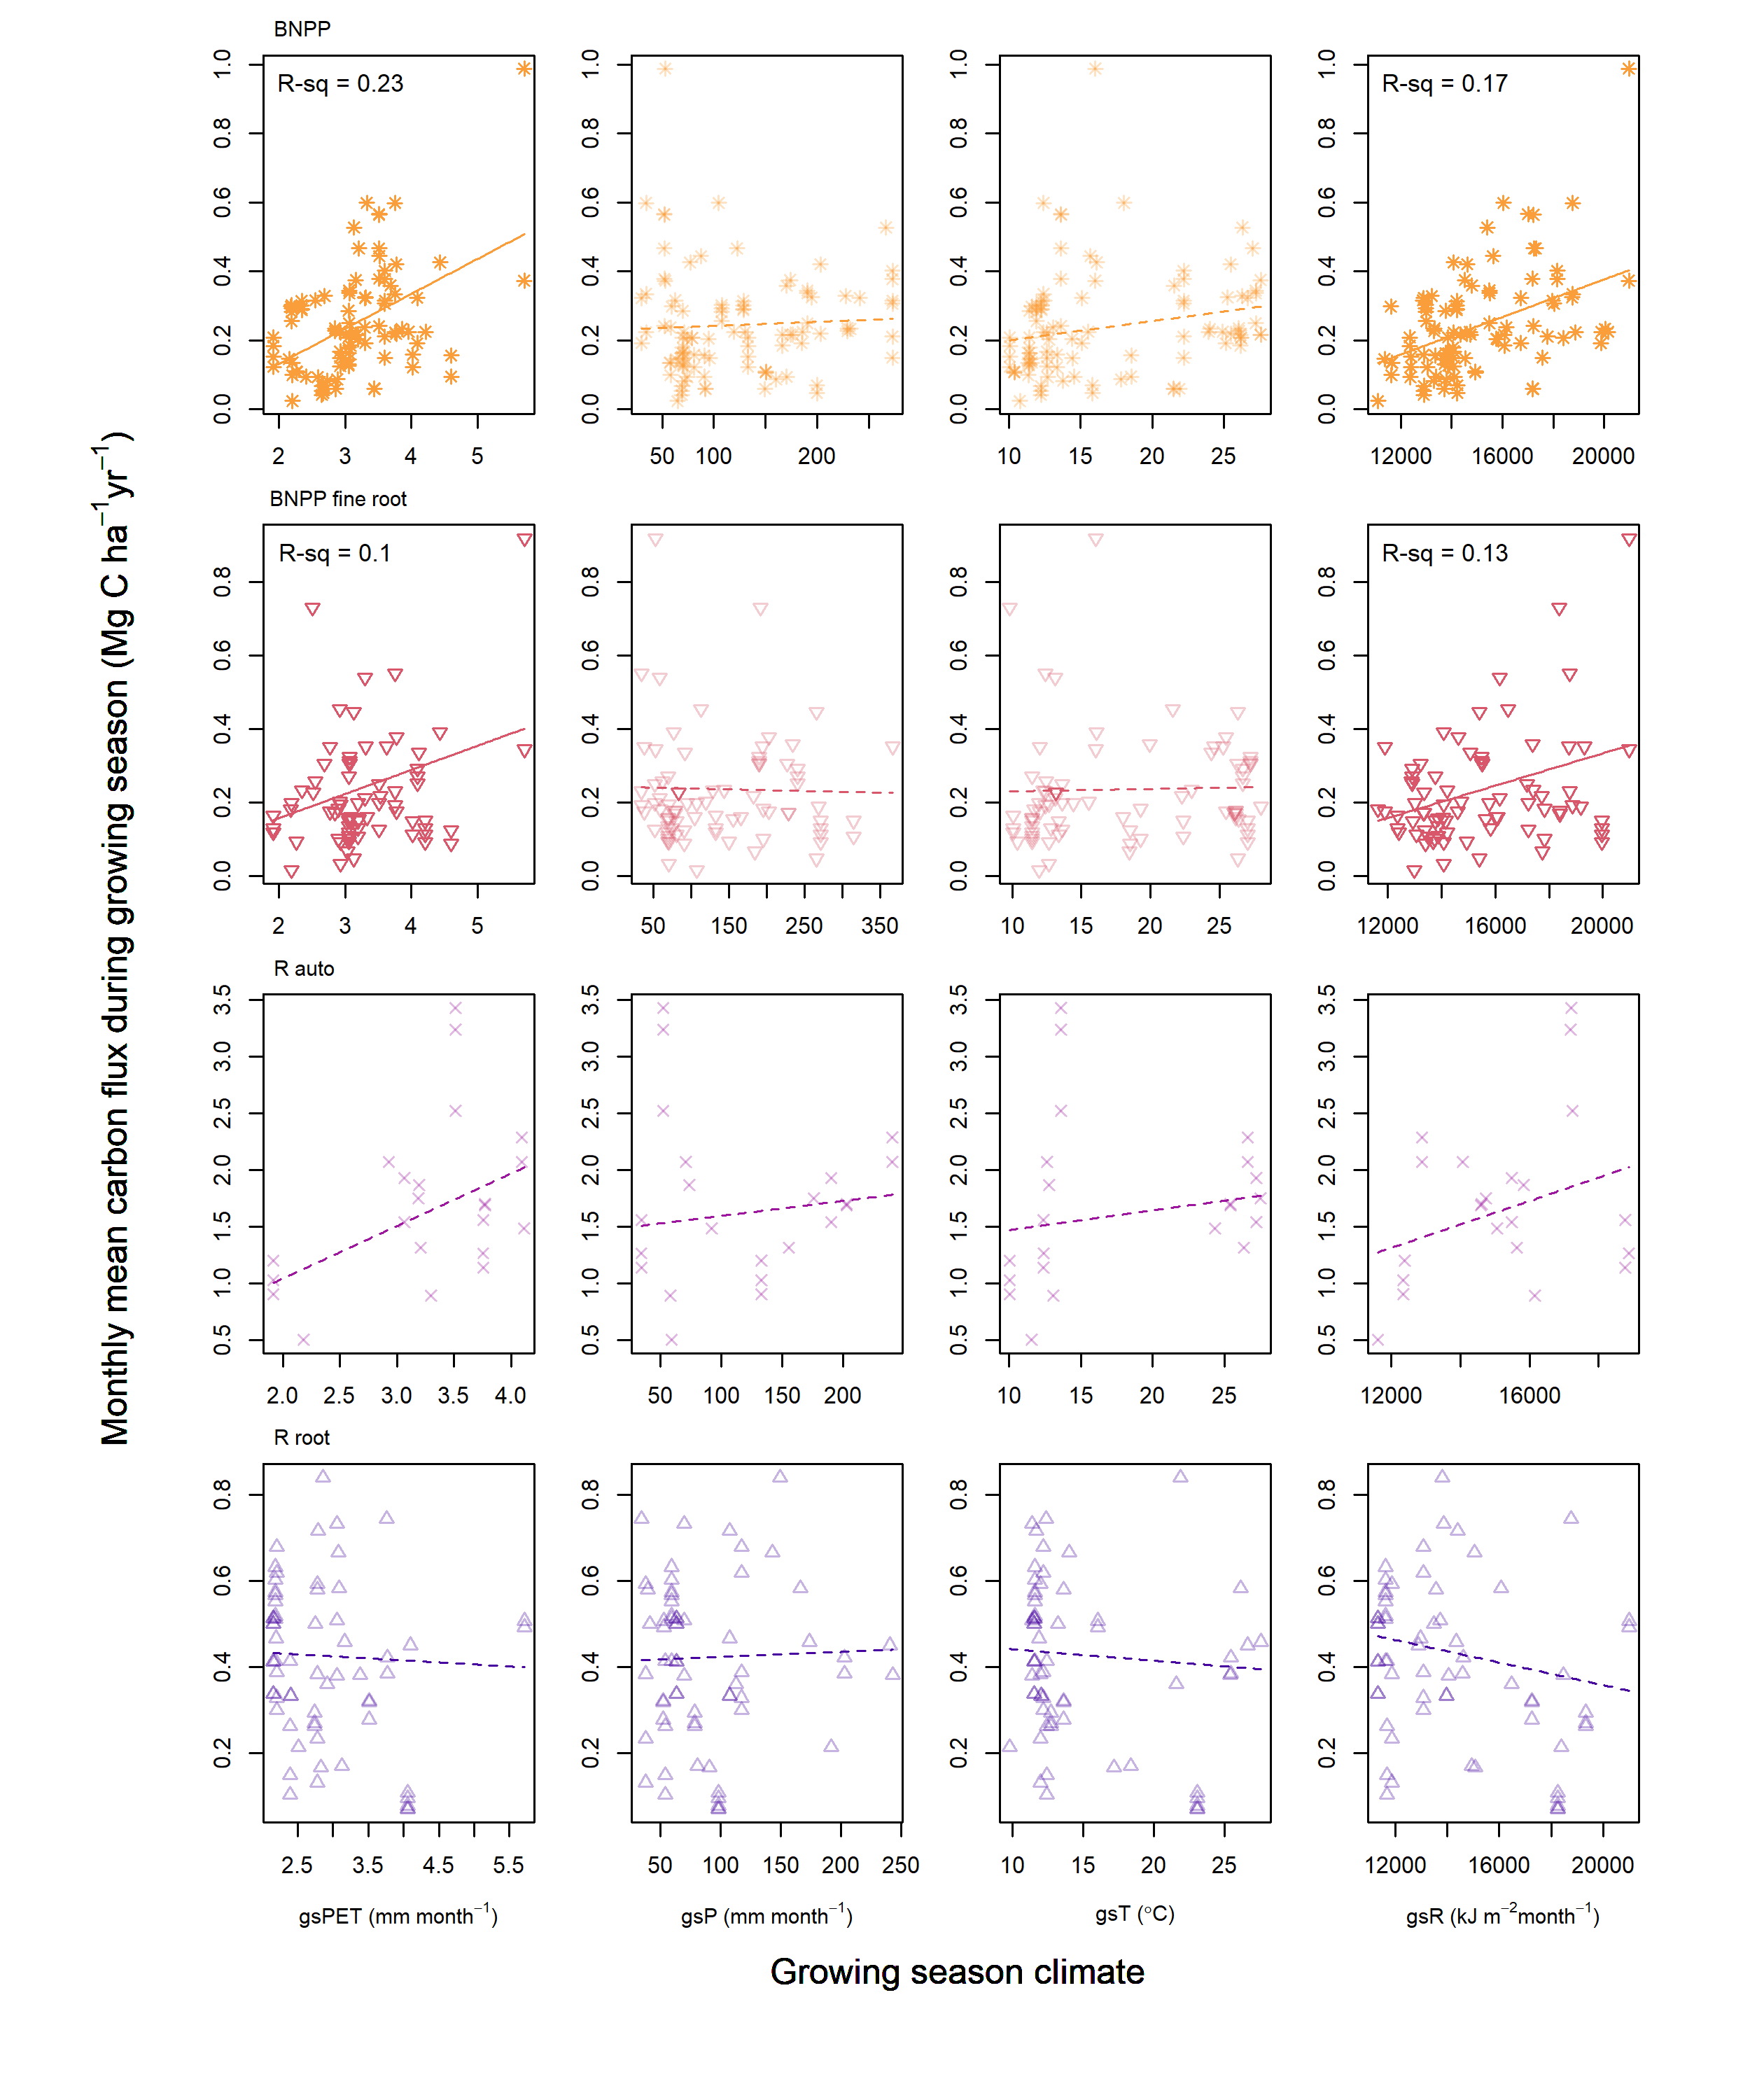
\includegraphics[width=1\linewidth]{tables_figures/gridded_growing_season2} \caption{Figure S8: Growing season length-standardized FACF in relation to mean growing season climate, part 2.}\label{fig:unnamed-chunk-14}
\end{figure}

\newpage

\begin{figure}[H]

{\centering 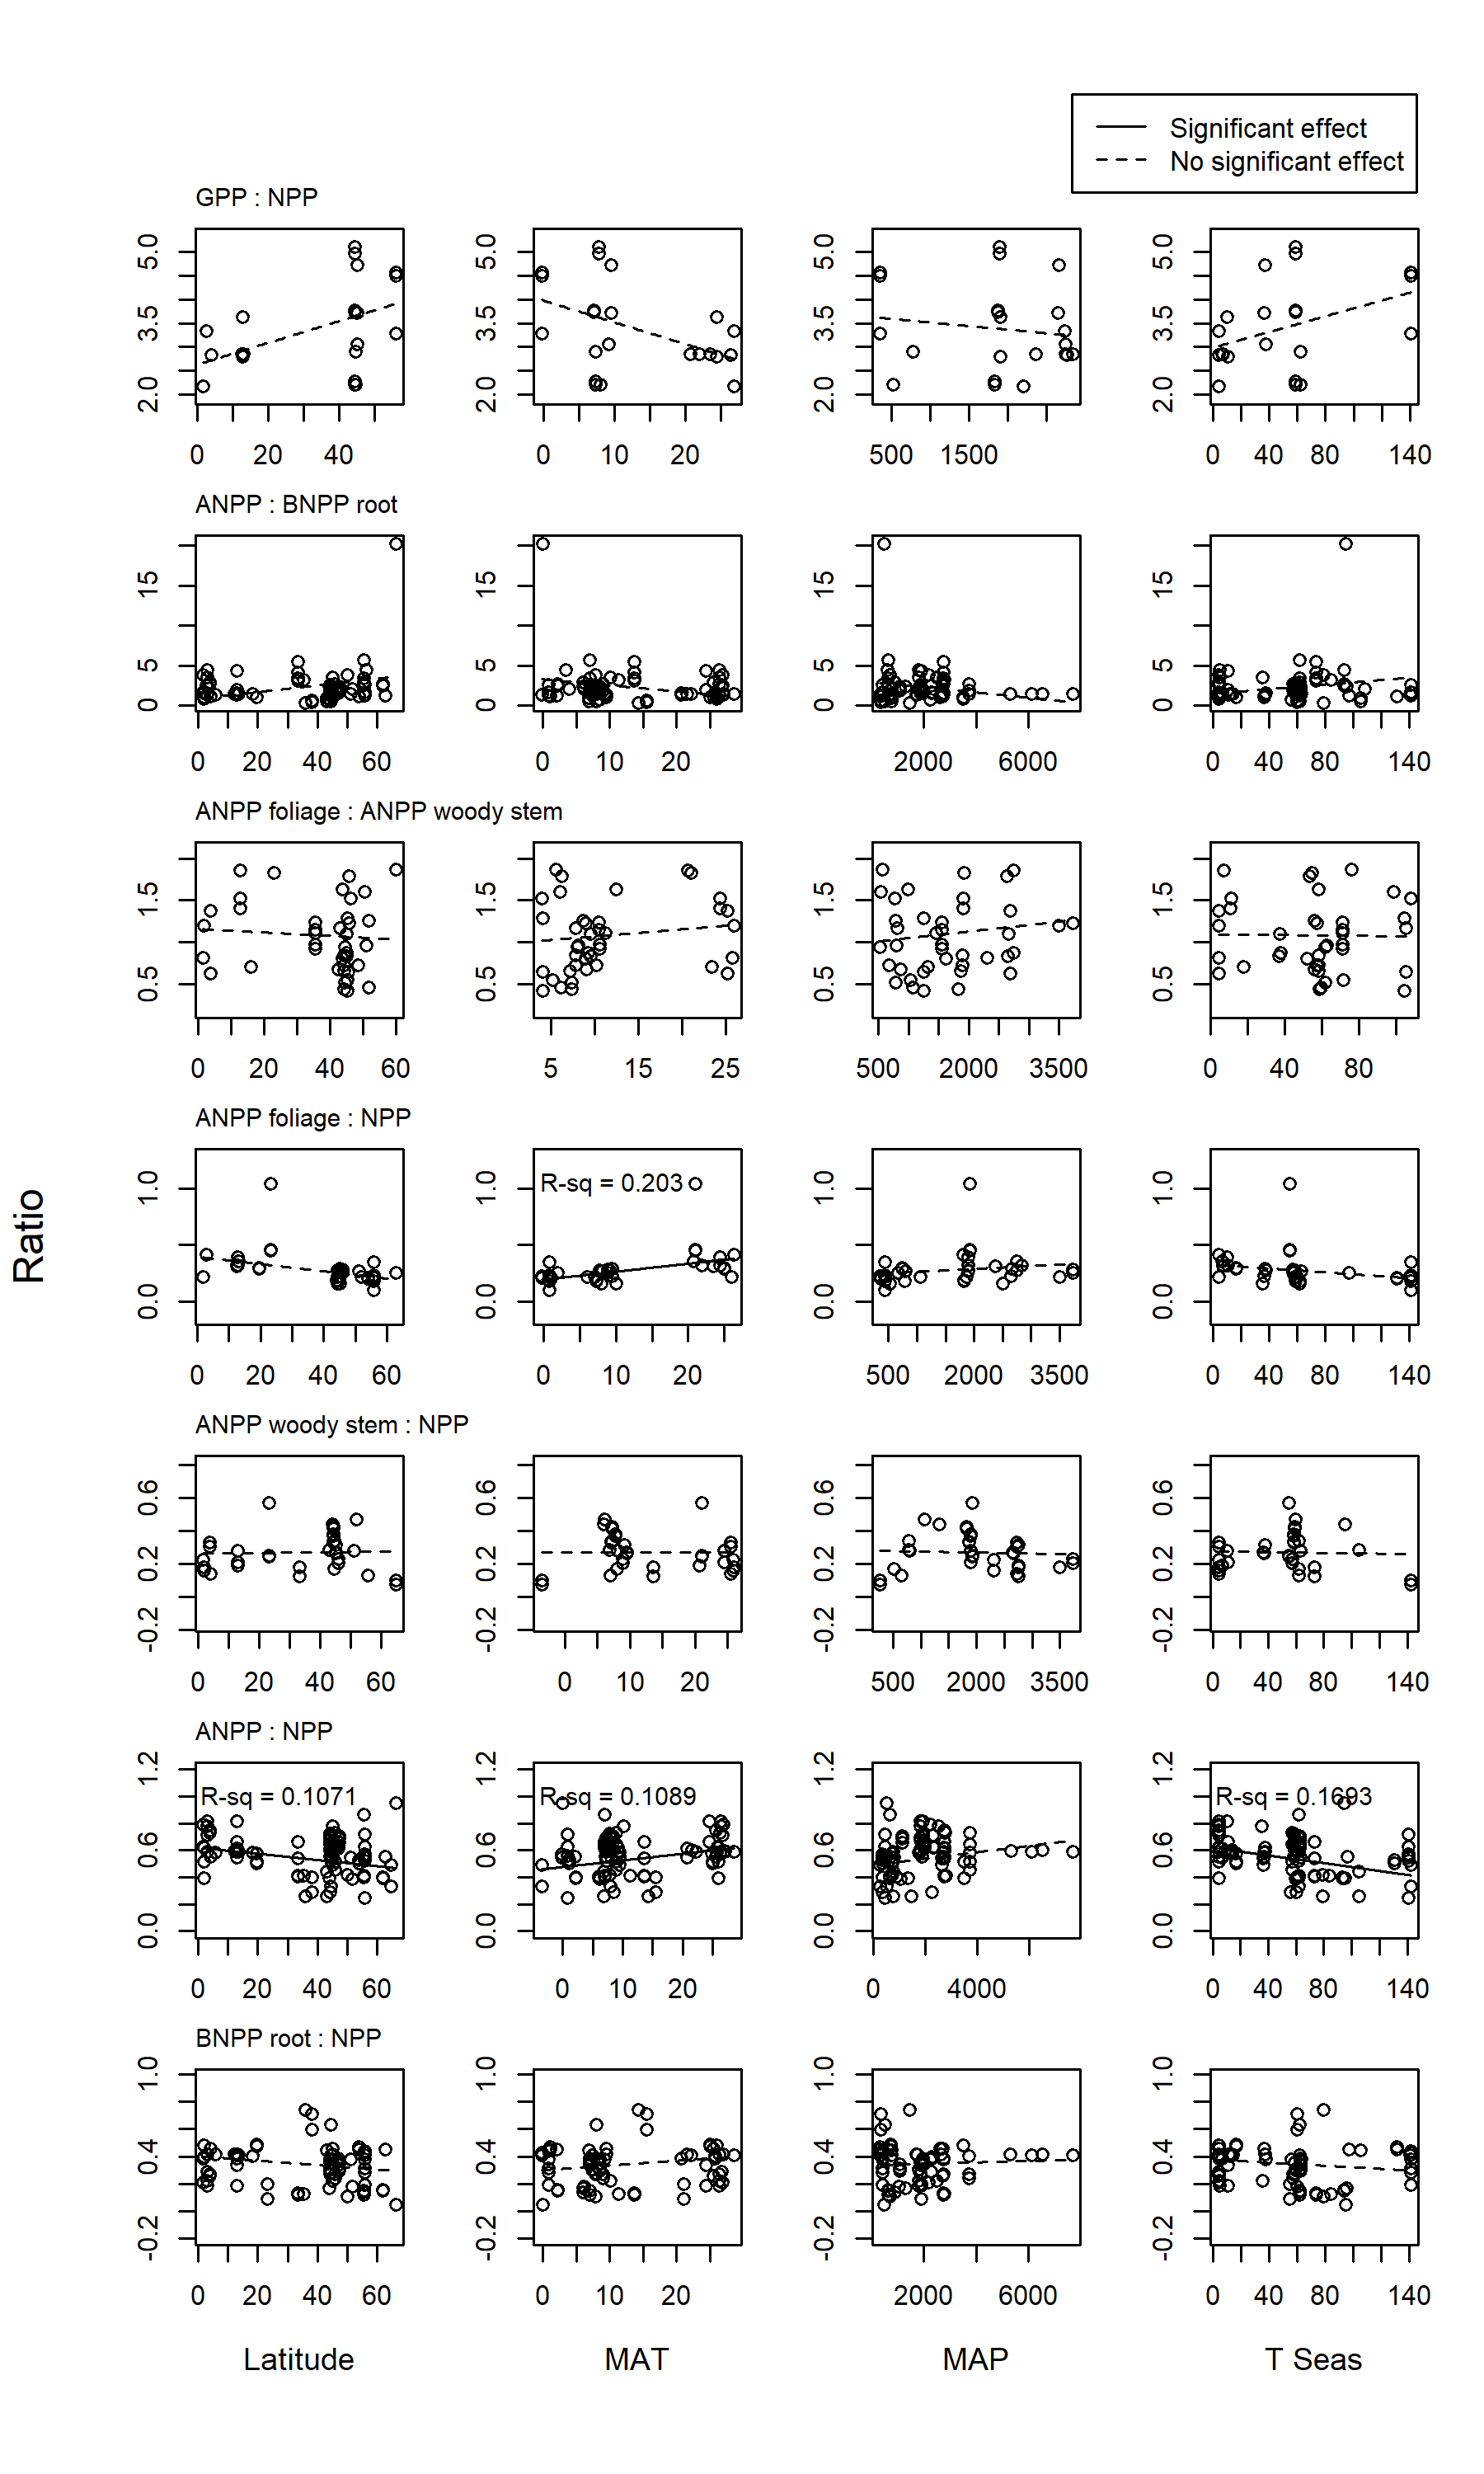
\includegraphics[width=1\linewidth]{tables_figures/ratio_grid_plots} 

}

\caption{Figure S9: Ratios among FACF as a function of latitude and climate variables}\label{fig:unnamed-chunk-15}
\end{figure}


\end{document}
